% Options for packages loaded elsewhere
\PassOptionsToPackage{unicode}{hyperref}
\PassOptionsToPackage{hyphens}{url}
\PassOptionsToPackage{dvipsnames,svgnames,x11names}{xcolor}
%
\documentclass[
]{article}

\usepackage{amsmath,amssymb}
\usepackage{iftex}
\ifPDFTeX
  \usepackage[T1]{fontenc}
  \usepackage[utf8]{inputenc}
  \usepackage{textcomp} % provide euro and other symbols
\else % if luatex or xetex
  \usepackage{unicode-math}
  \defaultfontfeatures{Scale=MatchLowercase}
  \defaultfontfeatures[\rmfamily]{Ligatures=TeX,Scale=1}
\fi
\usepackage{lmodern}
\ifPDFTeX\else  
    % xetex/luatex font selection
\fi
% Use upquote if available, for straight quotes in verbatim environments
\IfFileExists{upquote.sty}{\usepackage{upquote}}{}
\IfFileExists{microtype.sty}{% use microtype if available
  \usepackage[]{microtype}
  \UseMicrotypeSet[protrusion]{basicmath} % disable protrusion for tt fonts
}{}
\makeatletter
\@ifundefined{KOMAClassName}{% if non-KOMA class
  \IfFileExists{parskip.sty}{%
    \usepackage{parskip}
  }{% else
    \setlength{\parindent}{0pt}
    \setlength{\parskip}{6pt plus 2pt minus 1pt}}
}{% if KOMA class
  \KOMAoptions{parskip=half}}
\makeatother
\usepackage{xcolor}
\setlength{\emergencystretch}{3em} % prevent overfull lines
\setcounter{secnumdepth}{5}
% Make \paragraph and \subparagraph free-standing
\makeatletter
\ifx\paragraph\undefined\else
  \let\oldparagraph\paragraph
  \renewcommand{\paragraph}{
    \@ifstar
      \xxxParagraphStar
      \xxxParagraphNoStar
  }
  \newcommand{\xxxParagraphStar}[1]{\oldparagraph*{#1}\mbox{}}
  \newcommand{\xxxParagraphNoStar}[1]{\oldparagraph{#1}\mbox{}}
\fi
\ifx\subparagraph\undefined\else
  \let\oldsubparagraph\subparagraph
  \renewcommand{\subparagraph}{
    \@ifstar
      \xxxSubParagraphStar
      \xxxSubParagraphNoStar
  }
  \newcommand{\xxxSubParagraphStar}[1]{\oldsubparagraph*{#1}\mbox{}}
  \newcommand{\xxxSubParagraphNoStar}[1]{\oldsubparagraph{#1}\mbox{}}
\fi
\makeatother


\providecommand{\tightlist}{%
  \setlength{\itemsep}{0pt}\setlength{\parskip}{0pt}}\usepackage{longtable,booktabs,array}
\usepackage{calc} % for calculating minipage widths
% Correct order of tables after \paragraph or \subparagraph
\usepackage{etoolbox}
\makeatletter
\patchcmd\longtable{\par}{\if@noskipsec\mbox{}\fi\par}{}{}
\makeatother
% Allow footnotes in longtable head/foot
\IfFileExists{footnotehyper.sty}{\usepackage{footnotehyper}}{\usepackage{footnote}}
\makesavenoteenv{longtable}
\usepackage{graphicx}
\makeatletter
\newsavebox\pandoc@box
\newcommand*\pandocbounded[1]{% scales image to fit in text height/width
  \sbox\pandoc@box{#1}%
  \Gscale@div\@tempa{\textheight}{\dimexpr\ht\pandoc@box+\dp\pandoc@box\relax}%
  \Gscale@div\@tempb{\linewidth}{\wd\pandoc@box}%
  \ifdim\@tempb\p@<\@tempa\p@\let\@tempa\@tempb\fi% select the smaller of both
  \ifdim\@tempa\p@<\p@\scalebox{\@tempa}{\usebox\pandoc@box}%
  \else\usebox{\pandoc@box}%
  \fi%
}
% Set default figure placement to htbp
\def\fps@figure{htbp}
\makeatother
% definitions for citeproc citations
\NewDocumentCommand\citeproctext{}{}
\NewDocumentCommand\citeproc{mm}{%
  \begingroup\def\citeproctext{#2}\cite{#1}\endgroup}
\makeatletter
 % allow citations to break across lines
 \let\@cite@ofmt\@firstofone
 % avoid brackets around text for \cite:
 \def\@biblabel#1{}
 \def\@cite#1#2{{#1\if@tempswa , #2\fi}}
\makeatother
\newlength{\cslhangindent}
\setlength{\cslhangindent}{1.5em}
\newlength{\csllabelwidth}
\setlength{\csllabelwidth}{3em}
\newenvironment{CSLReferences}[2] % #1 hanging-indent, #2 entry-spacing
 {\begin{list}{}{%
  \setlength{\itemindent}{0pt}
  \setlength{\leftmargin}{0pt}
  \setlength{\parsep}{0pt}
  % turn on hanging indent if param 1 is 1
  \ifodd #1
   \setlength{\leftmargin}{\cslhangindent}
   \setlength{\itemindent}{-1\cslhangindent}
  \fi
  % set entry spacing
  \setlength{\itemsep}{#2\baselineskip}}}
 {\end{list}}
\usepackage{calc}
\newcommand{\CSLBlock}[1]{\hfill\break\parbox[t]{\linewidth}{\strut\ignorespaces#1\strut}}
\newcommand{\CSLLeftMargin}[1]{\parbox[t]{\csllabelwidth}{\strut#1\strut}}
\newcommand{\CSLRightInline}[1]{\parbox[t]{\linewidth - \csllabelwidth}{\strut#1\strut}}
\newcommand{\CSLIndent}[1]{\hspace{\cslhangindent}#1}

\makeatletter
\@ifpackageloaded{tcolorbox}{}{\usepackage[skins,breakable]{tcolorbox}}
\@ifpackageloaded{fontawesome5}{}{\usepackage{fontawesome5}}
\definecolor{quarto-callout-color}{HTML}{909090}
\definecolor{quarto-callout-note-color}{HTML}{0758E5}
\definecolor{quarto-callout-important-color}{HTML}{CC1914}
\definecolor{quarto-callout-warning-color}{HTML}{EB9113}
\definecolor{quarto-callout-tip-color}{HTML}{00A047}
\definecolor{quarto-callout-caution-color}{HTML}{FC5300}
\definecolor{quarto-callout-color-frame}{HTML}{acacac}
\definecolor{quarto-callout-note-color-frame}{HTML}{4582ec}
\definecolor{quarto-callout-important-color-frame}{HTML}{d9534f}
\definecolor{quarto-callout-warning-color-frame}{HTML}{f0ad4e}
\definecolor{quarto-callout-tip-color-frame}{HTML}{02b875}
\definecolor{quarto-callout-caution-color-frame}{HTML}{fd7e14}
\makeatother
\makeatletter
\@ifpackageloaded{caption}{}{\usepackage{caption}}
\AtBeginDocument{%
\ifdefined\contentsname
  \renewcommand*\contentsname{Table of contents}
\else
  \newcommand\contentsname{Table of contents}
\fi
\ifdefined\listfigurename
  \renewcommand*\listfigurename{List of Figures}
\else
  \newcommand\listfigurename{List of Figures}
\fi
\ifdefined\listtablename
  \renewcommand*\listtablename{List of Tables}
\else
  \newcommand\listtablename{List of Tables}
\fi
\ifdefined\figurename
  \renewcommand*\figurename{Figure}
\else
  \newcommand\figurename{Figure}
\fi
\ifdefined\tablename
  \renewcommand*\tablename{Table}
\else
  \newcommand\tablename{Table}
\fi
}
\@ifpackageloaded{float}{}{\usepackage{float}}
\floatstyle{ruled}
\@ifundefined{c@chapter}{\newfloat{codelisting}{h}{lop}}{\newfloat{codelisting}{h}{lop}[chapter]}
\floatname{codelisting}{Listing}
\newcommand*\listoflistings{\listof{codelisting}{List of Listings}}
\makeatother
\makeatletter
\makeatother
\makeatletter
\@ifpackageloaded{caption}{}{\usepackage{caption}}
\@ifpackageloaded{subcaption}{}{\usepackage{subcaption}}
\makeatother

\usepackage{bookmark}

\IfFileExists{xurl.sty}{\usepackage{xurl}}{} % add URL line breaks if available
\urlstyle{same} % disable monospaced font for URLs
\hypersetup{
  pdftitle={Unveiling the Complexity of Food Webs: A Comprehensive Overview of Definitions, Scales, and Mechanisms},
  pdfauthor={Tanya Strydom; Jennifer A. Dunne; Timothée Poisot; Andrew P. Beckerman},
  pdfkeywords={food web, network construction, scientific ignorance},
  colorlinks=true,
  linkcolor={blue},
  filecolor={Maroon},
  citecolor={Blue},
  urlcolor={Blue},
  pdfcreator={LaTeX via pandoc}}



\title{Unveiling the Complexity of Food Webs: A Comprehensive Overview
of Definitions, Scales, and Mechanisms}
\author{Tanya Strydom %
%
\textsuperscript{%
%
1%
}%
; Jennifer A. Dunne %
%
\textsuperscript{%
%
2%
}%
; Timothée Poisot %
%
\textsuperscript{%
3,%
4%
}%
; Andrew P. Beckerman %
%
\textsuperscript{%
%
1%
}%
}
\date{2024-11-14}

\usepackage{setspace}
\usepackage[left]{lineno}
\usepackage[letterpaper]{geometry}

\usepackage[nolists,noheads,markers]{endfloat}
\geometry{margin=2.5cm}

\begin{document}

\thispagestyle{empty}
{\bfseries\sffamily\Large Unveiling the Complexity of Food Webs: A
Comprehensive Overview of Definitions, Scales, and Mechanisms}
\vfil
Tanya Strydom %
%
\textsuperscript{%
%
1%
}%
; Jennifer A. Dunne %
%
\textsuperscript{%
%
2%
}%
; Timothée Poisot %
%
\textsuperscript{%
3,%
4%
}%
; Andrew P. Beckerman %
%
\textsuperscript{%
%
1%
}%

\vfil
{\small
\textbf{Abstract:} Food webs are a useful abstraction and representation
of the feeding links between species in a community and are used to
infer many ecosystem level processes. However, the different theories,
mechanisms, and criteria that underpin how a food web is defined, and
ultimately, constructed means that not all food webs are representing
the same ecological process at the same scale. Here we present a
synthesis of the different assumptions, scales, and mechanisms that are
used to define the different ecological networks ranging from metawebs
(an inventory of all potential interactions) to fully realised networks
(interactions that occur within a given community over a certain
timescale). Additionally we explicitly link the different network
representations to the broader methodological approaches (models) that
are used to construct them. In illuminating the assumptions, scales, and
mechanisms of network inference allows for a formal categorisation of
how to use networks to answer key ecological and conservation questions
as wel as defining clear guidelines to prevent unintentional misuse or
misinterpretation.
\vfil
\textbf{Keywords:} %
food web, network construction, %
scientific ignorance%
}
\clearpage
\setcounter{page}{1}
\doublespacing
\linenumbers


At the heart of modern biodiversity science are a set of concepts and
theories about biodiversity, stability, and function. These relate to
the abundance, distribution, and services that biodiversity provides,
and how biodiversity -- as an interconnected set of species -- responds
to multiple stressors. The interaction between species is one of the
fundamental building blocks of ecological communities, providing a
powerful abstraction that can help quantify, conceptualise, and
understand biodiversity dynamics, and ultimately, make predictions,
mitigate change, and manage services (Windsor et al., 2023). Such
network representations of biodiversity (including within species
diversity) are increasingly argued to be an asset to predictive ecology,
climate change mitigation, and resource management. With the argument
that characterising biodiversity in a network will afford a deeper
capacity to understand and predict the abundance, distribution,
dynamics, and services provided by multiple species facing multiple
stressors. However, there is a growing discourse around limitations to
the interpretation and applied use of networks (Blüthgen, 2010; Dormann,
2023), primarily as the result of shortcomings regarding the
conceptualisation of networks (Blüthgen \& Staab, 2024).

An `interaction network' can be defined and conceptualised in a myriad
of ways, which means that different networks embed different processes
(or determinants) of interactions, ultimately influencing the patterns
and mechanisms that are inferred (Proulx et al., 2005). The different
ways in which a network can be represented is the result of \emph{how}
the network is constructed, which itself rests on two pillars: the data
used to construct the network (of which there has been a plethora of
discussions as to the challenges relating to the scale and nature of
data collection/observation \emph{e.g.,} Blüthgen \& Staab, 2024;
Brimacombe et al., 2023; Moulatlet et al., 2024; Polis, 1991; Pringle \&
Hutchinson, 2020; Saberski et al., 2024) and the underlying theory as to
what drives the occurrence of interactions between species. The latter
represents an expression of mechanism and process that gives rise to the
patterns that emerge from collating interactions among species, and will
ultimately inform which data are deemed important in the determination
of interactions occurring. Each of these pillars carries with it a set
of practical, semantic and conceptual constraints that not only
influence progress in making network ecology more valuable and
potentially predictive, but help define the spatial, temporal, and
evolutionary scale of assumptions we make and the predictions we might
generate from different network representations.

In this perspective we aim to provide an overview of the different
\textbf{food web} representations, particularly how these relate to the
terminology used to define a food web, and how this influenced by both
the processes that determine interactions as well as how this relates to
the way in which we construct the resulting networks. An understanding
of the nuances of what different network representations are encoding
provides insights and conclusions about whether, when, and under what
conditions network representations of biodiversity can contribute to the
advancement of ecological theory and be of value in predictive ecology.
Specifically, we finish this perspective with an overview of fundamental
questions in ecology that we think can benefit from network thinking and
a proposal that such thinking can accelerate our capacity to predict the
impact of change on biodiverse communities.

\section{Setting the Scene: The Not So Basics of Nodes and
Edges}\label{sec-anatomy}

Defining a food web seems simple; it is the representation of feeding
interactions (edges) between species (nodes) in the form of a network,
however the definition of `edges' and `nodes', as well as the levels of
organization at which they are aggregated can take many forms Moulatlet
et al. (2024), which ultimately encodes a series of assumptions and
criteria within a network. An awareness of variance in the way a food
web can be defined is critical as a network (or its adjacency matrix) is
both the `object' from which inferences are made (\emph{e.g.,} the
interactions between species, or how the structure influences ecosystem
level processes) as well as the `product' of either the data collection
(Brimacombe et al., 2023) or prediction process (Banville et al., 2024).
One thus needs to be aware of both the criteria that is used to define
nodes and edges, and what processes or mechanisms the aggregation of the
two represents, as this will determine what the network can be used for.

\subsection{How do we define a node?}\label{how-do-we-define-a-node}

Although this may seem an elementary question in the context of food
webs --- a node \emph{should} represent a (taxonomic) species, the
reality is that nodes can often represent an aggregation of different
species - so called `trophic species' (Williams \& Martinez, 2000;
Yodzis, 1982) or segregation of species by life stages (Clegg et al.,
2018). Practical implications of how we are aggregating the nodes is
that the resolution may not always be `pixel perfect', which limits the
ability to make (taxonomic) species specific inferences (\emph{e.g.,}
does species \(a\) eat species \(b\)), however there is value in having
nodes that represent an aggregation of species, as the distribution of
the links between them are more meaningful in terms of understanding
energy flow and distribution within the system.

\subsection{What is captured by an
edge?}\label{what-is-captured-by-an-edge}

At its core, links within food webs can be thought of as a
representation of either feeding links between species - be that
realised (Pringle, 2020) or potential (Dunne, 2006), or links can
represent fluxes within a system \emph{e.g.,} energy transfer or
material flow as the result of the feeding links between species
(Lindeman, 1942). Fundamentally this means that the links within a
network represent different `currencies' (either the feasibility of a
link existing between two species or the energy that is moving through
the system) and how the links within a network are specified will
influence the resulting structure of the network. For example, taking a
food web that consists of links representing all \emph{potential}
feeding links for a community (\emph{i.e.,} a metaweb) will be
meaningless if one is interested in understanding the flow of energy
through the network as the links within a metaweb do not represent
environmental/energetic constraints, making them poor representations of
which interactions are \emph{realised} in a specific location (Caron et
al., 2024). In addition to the various ways of defining the links
between species pairs there are also a myriad of ways in which the links
themselves can be quantified. Links between species are often treated as
being present or absent (\emph{i.e.,} binary) but it is also possible to
use probabilities (Banville et al., 2024; which quantifies how likely an
interaction is to occur, Poisot, Cirtwill, et al., 2016) or continuous
measurements (which quantifies the strength of of an interaction, Berlow
et al., 2004).

\subsection{Network representations}\label{network-representations}

Broadly, networks can be thought of to fall into two different `types';
namely metawebs; traditionally defined as all of the \emph{potential}
interactions for a specific species pool (Dunne, 2006), and realised
networks; which is the subset of interactions in a metaweb that are
\emph{realised} for a specific community at a given time and place. The
fundamental difference between these two different network
representations is that a metaweb provides insight as to the viability
of an interaction between two species occurring and is a means to
identify links that are not ecologically plausible, \emph{i.e.,}
forbidden links (Jordano, 2016b), or provide an idea of the
\emph{complete} diet of a species (Strydom et al., 2023). In contrast
realised networks are highly localised and the links between species are
contingent on both the co-occurrence of species, the role of the
environment, and the population and community dynamics on predator
choice. In the context of definitions and semantics the links that are
represented by a metaweb and a realised network are different; links
that are absent in a metaweb can (conceptually although not always
practically) be treated as being truly absent, however links that are
absent in a realised network cannot be considered to be truly absent but
rather as absent due to the broader environmental/community context.
Importantly, a realised network is \emph{not} simply the downscaling of
a metaweb to a smaller scale (\emph{e.g.,} moving from the country to
the 1x1 km\textsuperscript{2} scale based on fine-scale species
co-occurrence) but rather represents a shift towards capturing the
higher level processes that determine the \emph{realisation} of an
interaction, \emph{i.e.,} the definition of an edges shifts from being
determined by interaction feasibility to that of energetic
choices/consequences. Thus, different network representations are
determined and constrained by different sets of assumptions as to what
the processes are that determine the presence/absence of an interaction
between two species as well as the resulting network structure.

\section{From Nodes and Edges to Scale, Context, and
Process}\label{sec-process}

The interplay between network representation and network (node and edge)
definition is primarily governed by the process(es) that determine the
interaction between species, however these processes are also scale and
context dependent. Here we start by introducing the five core processes
that determine either the feasibility or the realisation of
interactions, namely: evolutionary compatibility, co-occurrence,
abundance, profitability, and non-trophic interactions; while
simultaneously contextualising them within, and linking them to, the
different network representations Figure~\ref{fig-process}. We can think
of the different network representations to be conceptually analogous to
the fundamental and realised niche, whereby the metaweb represents the
`fundamental diet niche' of a species and a realised network represents
the `realised diet' of a species. Of course these processes do not
function in a vacuum and do interact with/influence one another, but it
is still beneficial to present them in a categorical manner as these
different processes are often the underpinning the logic in the
development of prediction/network models, the criteria for data
collection in the field, and the scale of organisation for which they
are relevant (species, population, or community).

\begin{figure}

\centering{

\pandocbounded{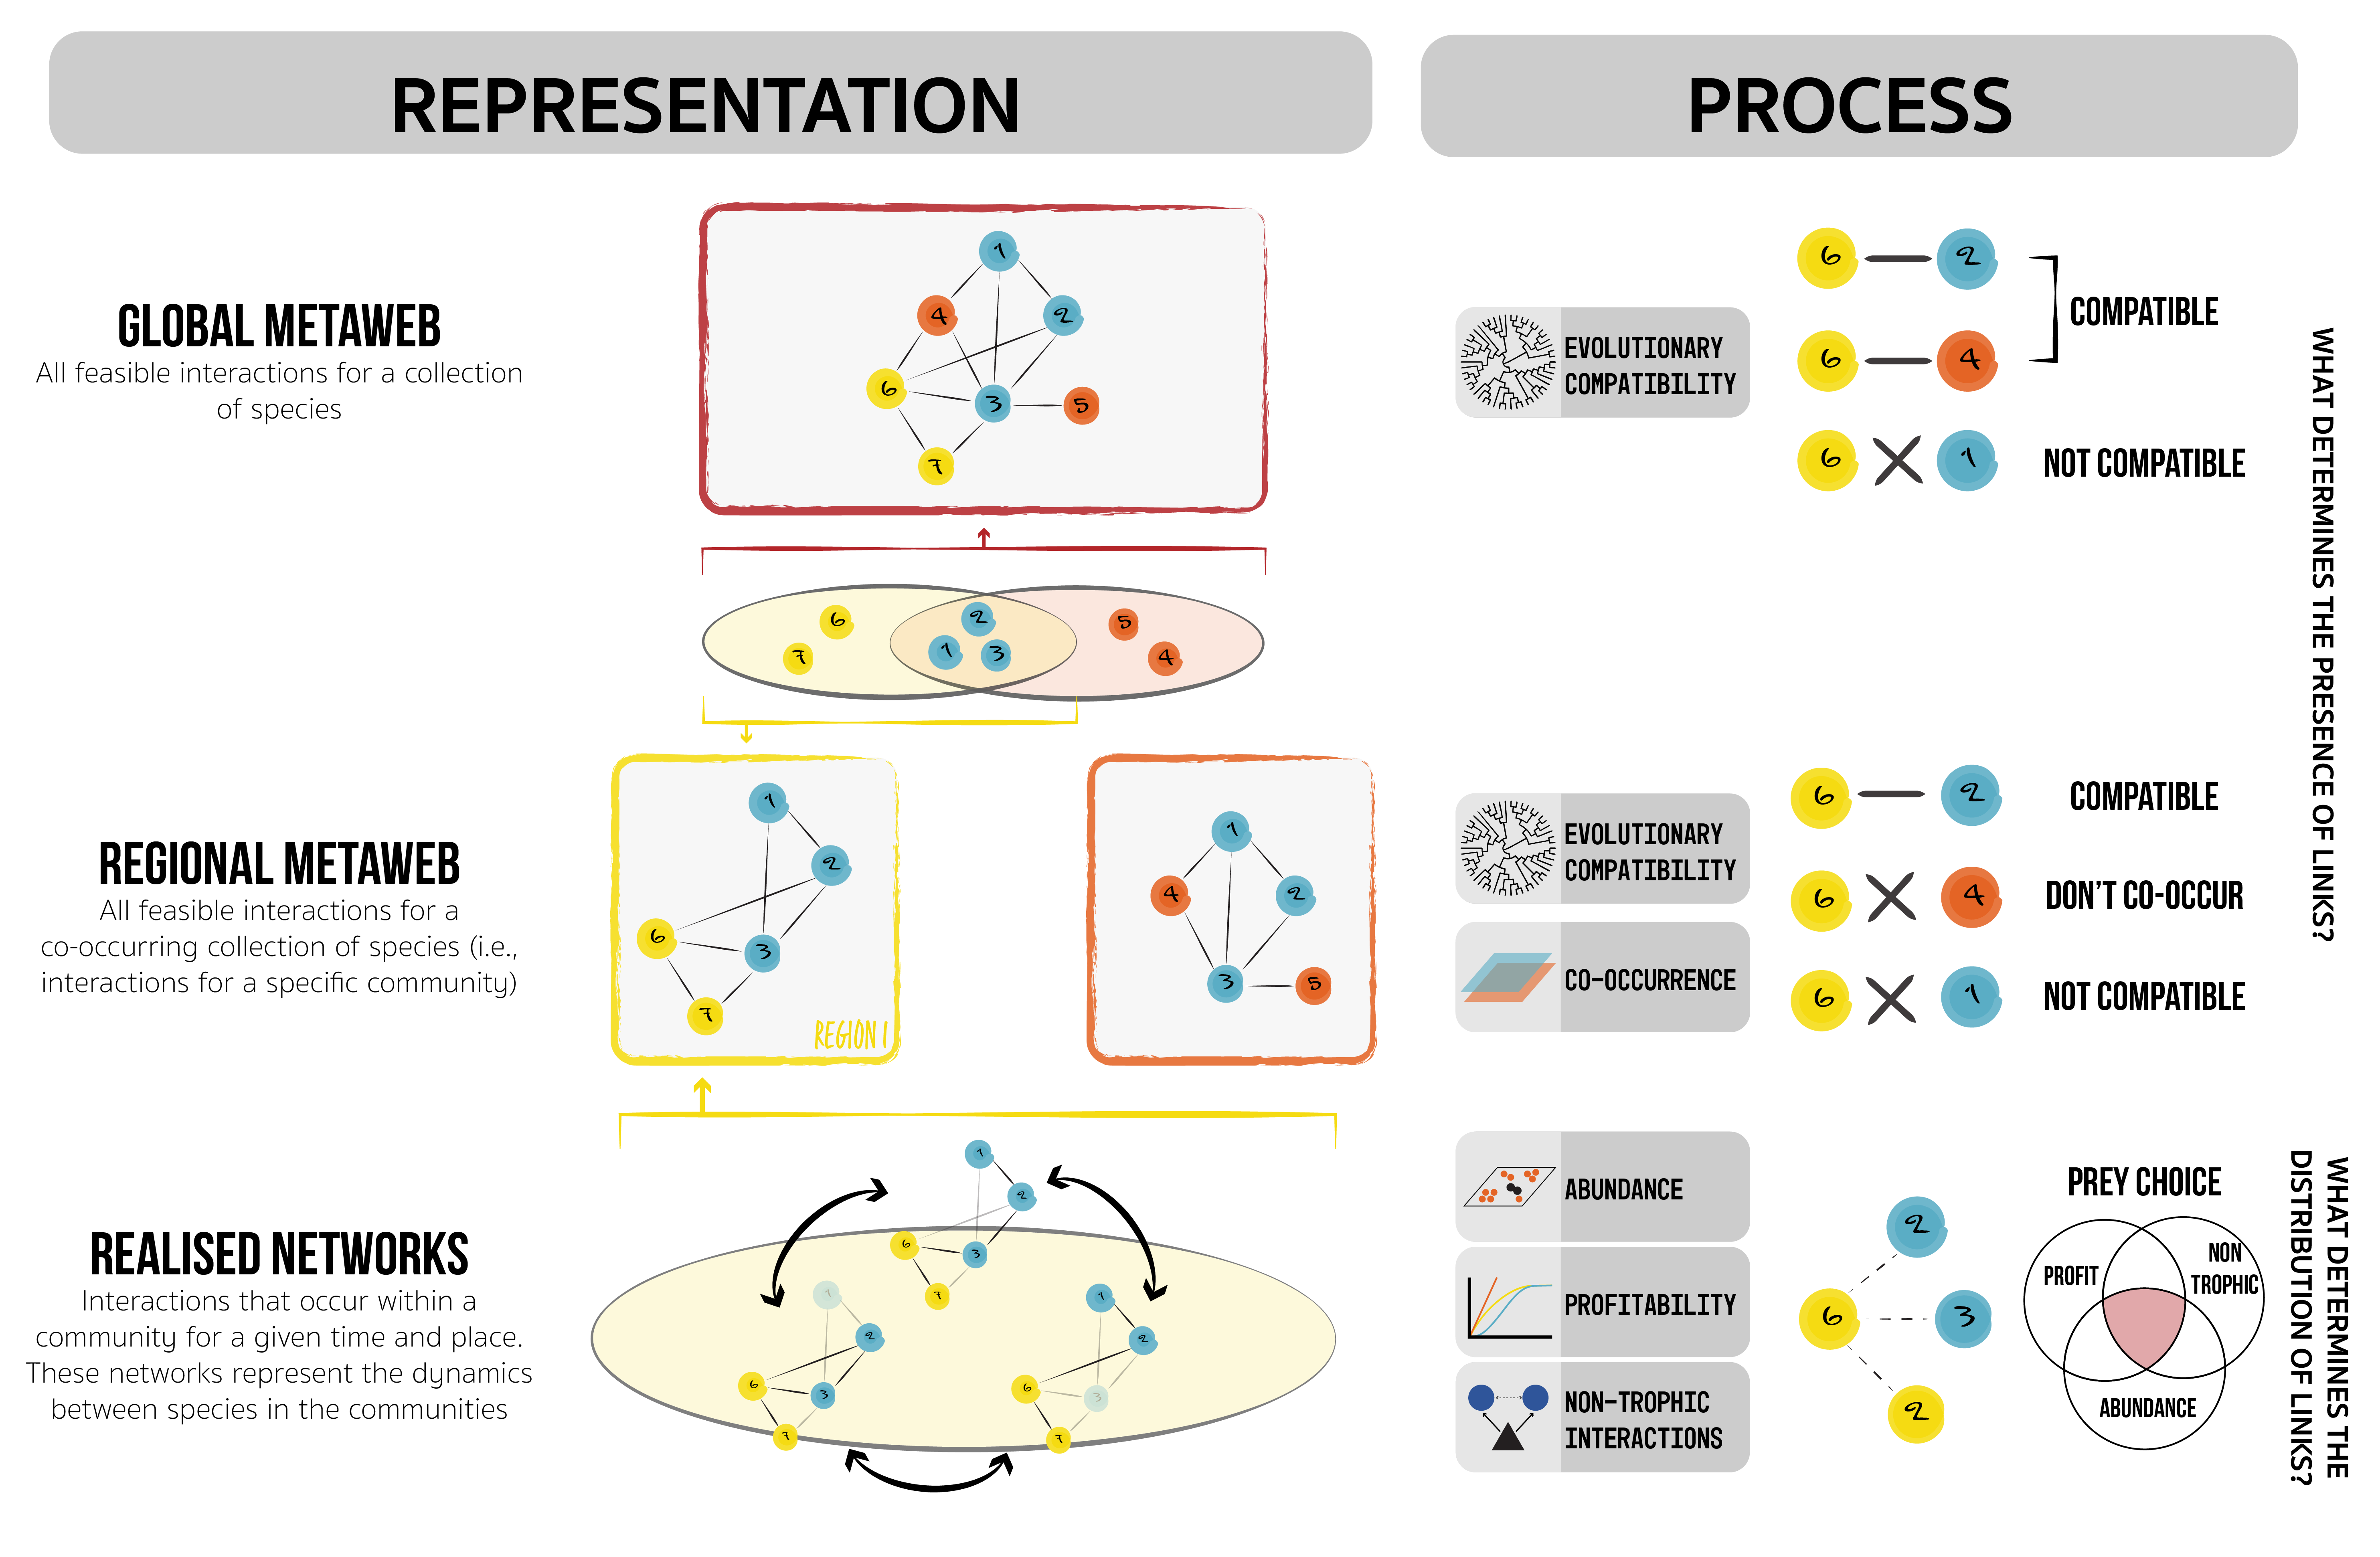
\includegraphics[keepaspectratio]{images/anatomy.png}}

}

\caption{\label{fig-process}Aligning the various processes that
determine interactions (right column) with the different network
representations (left column). First we start with a \textbf{global
metaweb} this network captures all possible interactions for a
collection of species in the global context. However within the global
environment different species occur in different regions (region one =
yellow and region 2 = orange), and it is possible to construct two
different metawebs (\textbf{regional metawebs}) for each region by
taking accounting for the co-occurrence patterns of the difference
species - as shown here we have two regions with some species (blue)
that are found in both regions and others endemic to either region one
(yellow) or region two (orange). However even within a region we do not
expect that all interactions to be realised but rather that there are
multiple configurations of the regional metaweb over both space and
time. The `state' of the different \textbf{realised networks} are
ultimately influenced not just by the co-occurrence of a species pair
but rather the larger community context such as the abundance of
different species, maximisation of energy gain, or indirect/higher order
interactions.}

\end{figure}%

\subsection{The processes that determine species
interactions}\label{the-processes-that-determine-species-interactions}

\textbf{Evolutionary compatibility}

There is compelling evidence that an interaction occurring between two
species is the result of their shared (co)evolutionary history (Dalla
Riva \& Stouffer, 2016; Gómez et al., 2010; Segar et al., 2020) which,
in the more proximal sense, is manifested as the `trait complementarity'
between two species (Benadi et al., 2022), whereby one species (the
predator) has the `correct' set of traits that allow it to chase,
capture, kill, and consume the other species (the prey). For species
pairs where this condition is not met the link is deemed to be
\emph{forbidden} (Jordano, 2016b); \emph{i.e.,} not physically possible
and will always be absent within a network. A network constructed on the
basis of evolutionary compatible links is most closely aligned with a
metaweb, although it would not be required that the species co-occur (as
shown in Figure~\ref{fig-process}), and arguably makes for a good
approximation of the `Eltonian niche' of species (Soberón, 2007).
Finally, one should be aware that it is possible to represent
evolutionary compatible interactions as either binary (possible vs
forbidden) or as a probability (Banville et al., 2024), where the
probability represents how likely the interaction between two species is
to be feasible.

\textbf{(Co)occurrence}

Although the outright assumption that because two species are
co-occurring it must mean that they are interacting is flawed (Blanchet
et al., 2020), it is of course impossible for two species to interact
(at least in terms of feeding links) if they are not co-occurring in
time and space. Thus, although co-occurrence data alone is insufficient
to build an accurate and ecologically meaningful representation of
\emph{feeding links} it is still a critical process that determines the
realisation of feeding links and allows us to constrain a global metaweb
to only consider `realised' communities (Dansereau et al., 2024) and an
understanding of the intersection of species interactions and their
co-occurrence (\emph{sensu} a fusion of the the Grinnellian and Eltonian
niches niche, Gravel et al. (2019)) is meaningful when one is operating
in the space of trying to determine the distribution of a species
(Higino et al., 2023; Pollock et al., 2014).

\textbf{Abundance}

The abundance of the different species within the community is thought
to influence the realisation of feeding links primarily in two ways.
Firstly, there is the argument that the structure of networks (and the
interactions that they are composed of) are driven \emph{only} by the
abundance of the different species and that interactions are not
contingent on there being any compatibility (trait matching) between
them, \emph{sensu} neutral processes (Canard et al., 2012; Momal et al.,
2020). However, a more ecologically sound assumption would be that the
abundance of different prey species will influence the distribution of
links in a network (Vázquez et al., 2009), by influencing which prey are
targeted or preferred by the predator as abundance influences factors
such as the likelihood of two species (individuals) meeting (Banville et
al., 2024; Poisot et al., 2015), or in the dynamic sense will influence
the persistence of viable populations.

\textbf{Profitability (energetics)}

Ultimately, predator choice is underpinned by the energetic cost-benefit
(profitability) of trying to catch, kill, and consume prey (where a
predator will optimise energy intake while minimising handling and
search time (energy cost)), and is well described within both optimal
foraging (Pyke, 1984) and metabolic theory (Brown et al., 2004). The
energetic cost of feeding is determined by both the energy content as
well as the density (abundance) of prey (as this influences search
time), and a predator will opt to select the prey type that will be most
profitable. Additional work on on understanding the energetic cost that
the environment imposes on an individual (Cherif et al., 2024) as well
as the way a predator uses the landscape to search for prey (Pawar et
al., 2012) brings us closer to accounting for the energetic cost of
realising feeding links.

\textbf{Non-trophic interactions}

Perhaps not as intuitive when thinking about the processes that
determine feeding links is accounting for the ability of non-trophic
interactions (such as competition) to modify either the realisation or
strength of trophic interactions (Golubski \& Abrams, 2011; Pilosof et
al., 2017). Non-trophic interactions can modify interactions either
`directly' \emph{e.g.,} predator \emph{a} outcompetes predator \emph{b}
or `indirectly' \emph{e.g.,} mutualistic/facilitative interactions will
alter the fine-scale distribution and abundance of species as well as
their persistence (Buche et al., 2024; Kéfi et al., 2012, 2015). The
`unobservable' nature of non-trophic interactions makes them a challenge
to quantify, however their importance in network dynamics (Staniczenko
et al., 2010) as well as cascading effects (\emph{e.g.,} Kamaru et al.,
2024) should not be overlooked.

\subsection{Contextualising the processes that determine species
interactions}\label{contextualising-the-processes-that-determine-species-interactions}

It should be self evident that the different processes discussed above
will ultimately influence the realisation of interactions as well as the
structure of a network, however they are acting at different scales of
organisation. Both the \textbf{co-occurrence} and the
\textbf{evolutionary compatibility} are valid at the scale of the
species pair of interest, that is the \emph{possibility} of an
interaction being present/absent is assessed at the pairwise level and
one is left with a `list' of interactions that are present/absent.
Although it is possible to build a network (\emph{i.e.,} metaweb) from
this information it is important to be aware that the structure of this
network is not constrained by real-world dynamics or conditions
(\emph{i.e.,} the community context), and so just because species are
able to interact does not mean that they will (Poisot et al., 2015). In
order to construct a network who's structure is a closer approximation
of reality (localised interactions) one needs to take into consideration
the properties of the community as a whole and information about the
individuals it is comprised of (Quintero et al., 2024), which requires
more data at the community scale, which, as shown in
Figure~\ref{fig-process}, is encapsulated by the intersections of
species \textbf{abundance}, \textbf{profitability}m and the role of
\textbf{non-trophic interactions}.

\section{Network construction is
nuanced}\label{network-construction-is-nuanced}

The act of constructing a `real world' network will ultimately be
delimited by its intended use, however the reality is that the empirical
collection of interaction data is both costly and challenging to execute
(Jordano, 2016a, 2016b), especially if one wants to capture \emph{all}
aspects of the processes discussed in Section~\ref{sec-process} (owing
to the different time and spatial scales they may be operating at). Thus
we often turn to models to either predict networks (be that the
interaction between two species, or network structure (Strydom et al.,
2021)), or as a means to identify missing interactions (gap fill) within
an existing empirical dataset (\emph{e.g.,} Biton et al., 2024; Dallas
et al., 2017; Stock, 2021), and so for the purpose of this discussion
network construction will be synonymous with using a model as a means to
represent or predict a network. That is not to say that there is no need
for empirical data collection, but rather that using a model for food
web prediction (or reconstruction) is a more feasible approach as it
allows us to make inferences about interactions that are not happening
in the `observable now' (Strydom et al., 2021), and has the added
benefit that one is able to explicitly account for uncertainty within
the network construction process (Banville et al., 2024). Most
importantly different models have different underlying philosophies,
this allows isolate and operate within one (or a few) of the processes
discussed in Section~\ref{sec-process}, and better sets us up to
understand how different processes determine interactions (Song \&
Levine, 2024; Stouffer, 2019). Here we will introduce the three
different types of network representations (metawebs, realised networks,
and structural networks), how they link back to (and encode) the
different processes determining interactions Figure~\ref{fig-process},
and broadly discuss some of the modelling approaches that are used to
construct these different network types. This is paralleled by a
hypothetical case study (Box 1) where we showcase the
utility/applicability of the different network representations in the
context of trying to understand the feeding dynamics of a seasonal
community.

\begin{tcolorbox}[enhanced jigsaw, colframe=quarto-callout-note-color-frame, opacitybacktitle=0.6, rightrule=.15mm, left=2mm, coltitle=black, opacityback=0, breakable, leftrule=.75mm, title=\textcolor{quarto-callout-note-color}{\faInfo}\hspace{0.5em}{Box 1 - Why we need to aggregate networks at different scales: A
hypothetical case study}, toprule=.15mm, bottomtitle=1mm, colback=white, toptitle=1mm, colbacktitle=quarto-callout-note-color!10!white, titlerule=0mm, bottomrule=.15mm, arc=.35mm]

Although it might seem most prudent to be predicting, constructing, and
defining networks that are the closest representation of reality there
are pros and cons of constructing both realised networks as well as
metawebs. Let us take for example a community that experiences a degree
of species turnover between seasons. In this community we expect species
to be either present or absent depending on the season (\emph{i.e.,}
changes in co-occurrence) as well as some species exhibiting seasonal
shifts in their diets (be that due to changes in species occurrence or
predator choice). If one were to construct a metaweb that disregards
these season shifts (\emph{i.e.,} a global metaweb) it is clear that
these finer nuances would be lost. It is of course possible to construct
either smaller metawebs for the different seasonal communities (thereby
capturing the changes in community diversity), or realised networks for
each season (to capture diet or ecosystem process shifts \emph{e.g.,}
Schwarz et al. (2020)). However, these small-scale networks lack the
context of the bigger picture that is available at the metaweb - that is
it gives us a more holistic idea of the entire diet range of a specific
species, which is important when one needs to make
conservation-based/applied decisions (\emph{e.g.,} conserving the entire
diet of a species and not just seasonal prey items) as well as providing
information on interactions that may be possible regardless of the
environmental/community context (species may have the capacity to
consume certain prey items but do not do so due to local conditions).
With this is mind let us see how the different network aggregations can
be used:

\textbf{1. A global metaweb:} Knowledge of the entire diet breadth of a
species is valuable especially in terms of understanding how a species
will respond to changes in the community - \emph{e.g.}
invasions/rewilding scenarios (where does the new species `fit' within
the network?) as well as potential capacity to shift its diet. There is
also the argument that a metaweb will allow us to identify species that
act as links across the landscape.

\textbf{2. A seasonal metaweb:} Knowledge at the finer scale is also
valuable to understand and provide insight on the differences in diets
between seasons (and identify key species within the network in
different environments).

\textbf{3. A realised network:} Provide insight as to the different
network configurations for a given time and place, which is a better
approximation of the energy flows/ecosystem processes as they are
occurring (that is the \emph{structure} of the network is also
meaningful). A realised network will also allow one to detect more
nuanced shifts diet - \emph{i.e.,} not only changes in links due to
species turnover between seasons.

\end{tcolorbox}

\subsection{Models that predict metawebs (feasible
interactions)}\label{models-that-predict-metawebs-feasible-interactions}

This is perhaps the most developed group of models; with a variety of
approaches having been developed that typically determine the
feasibility of an interaction using the trait compatibility between
predator and prey (\emph{i.e.} their evolutionary compatibility) to
determine `feeding rules' (Morales-Castilla et al., 2015). These feeding
rules are broadly elucidated in two different ways; mechanistic feeding
rules can be explicitly defined and applied to a community (Dunne et
al., 2008; Roopnarine, 2017; \emph{e.g.,} Shaw et al., 2024) or they are
inferred from a community for which there are interaction data and the
`rules' are then applied to a different community (Caron et al., 2022;
Cirtwill et al., 2019; Desjardins-Proulx et al., 2017; Eklöf et al.,
2013; Llewelyn et al., 2023; Pichler et al., 2020; Strydom et al., 2022;
\emph{e.g.,} Strydom et al., 2023). The fundamental difference between
these two model groups is that `mechanistic models' rely on expert
knowledge and make explicit assumptions on trait-feeding relationships,
whereas the `pattern finding' models are dependent on existing datasets
from which to elucidate feeding rules. These models are useful for
determining all feasible interactions for a specific community, and
owing to the availability of empirical interaction datasets (Gray et
al., 2015; \emph{e.g.,} Poelen et al., 2014; Poisot, Baiser, et al.,
2016), as well as the development of model testing/benchmarking tools
(Poisot, 2023), means that these models can be validated and (with
relative confidence) be used to construct first draft networks for
communities for which we have no interaction data (Strydom et al.,
2022), and are valuable not only in data poor regions but also for
predicting interactions for `unobservable' communities \emph{e.g.,}
prehistoric networks (Dunhill et al., 2024; Fricke et al., 2022; Yeakel
et al., 2014) or future, novel community assemblages. Importantly
metawebs are inherently `static' in the sense that they are \emph{not}
able to capture dynamic processes (since the notion of feasibility is
all or nothing), however they provide a bigger picture context
(\emph{e.g.,} understanding the \emph{entire} diet breadth of a species)
and often require little data to construct.

\subsection{Models that predict realised networks (realised
interactions)}\label{models-that-predict-realised-networks-realised-interactions}

In order to construct realised networks models need to incorporate
\emph{both} the feasibility of interactions (\emph{i.e.,} determine the
entire diet breadth of a species) as well as then determine which
interactions are realised (\emph{i.e.,} incorporate the `cost' of
interactions). As far as we are aware there is no model that explicitly
accounts for both of these `rules' (although see Olivier et al. (2019))
and rather \emph{only} account for processes that determine the
realisation of an interaction (\emph{i.e.,} abundance, predator choice,
or non-trophic interactions). Although the use of allometry \emph{i.e.,}
body size (Beckerman et al., 2006; \emph{e.g.,} Valdovinos et al., 2023;
White et al., 2007; Yodzis \& Innes, 1992) may represent a first step in
capturing `evolutionary compatibility' alongside more energy (predator
choice) driven processes we still need to account for other traits that
determine feeding compatibility (\emph{e.g.,} Van De Walle et al., 2023
show how incorporating prey defensive properties alongside body size
improves predictions). In terms of constructing realised networks, diet
models (Beckerman et al., 2006; Petchey et al., 2008) have been used
construct networks based on both predator choice (as determined by the
handling time, energy content, and predator attack rate) as well as
abundance (prey density) and progress has also been made in
understanding the compartmentation of energy in networks and how this
influences energy acquisition (Krause et al., 2003; Wootton et al.,
2023). As realised networks are are build on the concept of dynamic
processes (the abundance of species will always be in flux) these
networks are valuable for understanding the behaviour of networks over
time or their response to change (Curtsdotter et al., 2019; Delmas et
al., 2017; Lajaaiti et al., 2024). However, they are `costly' to
construct (requiring data about the entire community as it is the
behaviour of the system that determines the behaviour of the part) and
also lack the larger diet niche context afforded by metawebs.

\subsection{Models that predict structure (interaction
agnostic)}\label{models-that-predict-structure-interaction-agnostic}

Although we identify mechanisms that determine species interactions in
Section~\ref{sec-process} not all models that are used to predict
networks explicitly operate at the `process' level, but rather represent
the \emph{structure} of a network based on a series of \emph{a priori}
assumptions as to the distribution of links between (typically trophic
not taxonomic) species. These models operate by parametrising an aspect
of the network structure, (\emph{e.g.,} the niche model (Williams \&
Martinez, 2000) makes an assumption as to the expected connectance of
the network,although see Allesina \& Pascual (2009) for a parameter-free
model) or alternatively uses structural features of an exiting
\emph{realised} network (\emph{e.g.,} stochastic block model, Xie et al.
(2017)). Importantly these structural models do not make species
specific predictions (they are usually species agnostic and treat nodes
as trophic species) and so cannot be used to determine if an interaction
is either possible \emph{or} realised between two species (\emph{i.e.,}
one cannot use these models to determine if species \(a\) eats species
\(b\)). Although this means this suite of models are unsuitable as tools
for predicting species-specific interactions, they have been shown to be
sufficient tools to predict the structure of networks (Williams \&
Martinez, 2008), and provide a data-light (the models often only require
species richness) but assumption heavy (the resulting network structure
is determined by an assumption of network structure) way to construct a
network.

\section{Making Progress with
Networks}\label{making-progress-with-networks}

\subsection{Further development of models and
tools}\label{further-development-of-models-and-tools}

There has been a suite of models that have been developed to predict
feeding links, however we are lacking in tools that are explicitly
taking into consideration estimating both the feasibility as well as
realisation of links, \emph{i.e.,} both interactions and structure
simultaneously (Strydom et al., 2021). This could be addressed either
through the development of tools that do both (predict both interactions
and structure), or to develop an ensemble modelling approach (Becker et
al., 2022; Terry \& Lewis, 2020) or tools that will allow for the
downsampling of metawebs into realised networks (\emph{e.g.,}
Roopnarine, 2006). Additionally, although realised networks are more
closely aligned with capturing interaction strength we lack models that
allow us to quantify this (Strydom et al., 2021; Wells \& O'Hara, 2013).
In addition to the more intentional development of models we also need
to consider the validation of these models, there have been developments
and discussions for assessing how well a model recovers pairwise
interactions (Poisot, 2023; Strydom et al., 2021), although their are
still challenges related to the completeness of the datasets that are to
be used for validation, specifically the challenge of dealing with
false-negatives (Catchen et al., 2023). In terms of validating the
predicted structure of networks, we still lack clear set of guidelines
for benchmarking the ability of models to recover structure (Allesina et
al., 2008).

\subsection{At what scale should we be predicting and using
networks?}\label{at-what-scale-should-we-be-predicting-and-using-networks}

The appropriate level of aggregation for a `network' is an emerging
discussion within the field (Estay et al., 2023; Moulatlet et al., 2024;
Saberski et al., 2024), and perhaps presents the biggest challenge if we
want to understand how different processes determine interactions
(Saravia et al., 2022), as well as identify the appropriate networks for
different research questions Figure~\ref{fig-future}. Thus we need an
understanding of not only how time and scale influence the
interpretation of networks (Blüthgen \& Staab, 2021; Morales \& Vázquez,
2008), but how this is in turn influenced by the type of network
representations used. Space influences both network properties (Galiana
et al., 2018), as well as dynamics (Fortin et al., 2021; Rooney et al.,
2008), and time has implications when it comes to accounting for
seasonal turnover in communities (Brimacombe et al., 2021; Laender et
al., 2010) as well as thinking about co-occurrence, particularly the
records that are used to determine co-occurrence (Brimacombe et al.,
2024). Although multilayer networks may allow us to encode the nuances
of space and time (Hutchinson et al., 2019) we still need to understand
the implications of \emph{e.g.,} constructing networks that are not at
ecologically but rather politically relevant scales (Strydom et al.,
2022) and what the implications of this disconnect may be.

\subsection{Making use of the different network
representations}\label{making-use-of-the-different-network-representations}

It should be clear that there is a high degree of interrelatedness and
overlap between the way in which a network is constructed (modelled or
predicted) and the process(es) that it captures
Figure~\ref{fig-process}, these are encoded (embedded) within the
network representation and ultimately influences how the network can and
should be used (Berlow et al., 2008; Petchey et al., 2011), with
different network representations yielding different interpretations of
processes (Keyes et al., 2024). It is probably both this nuance as well
as a lack of clear boundaries and guidelines as to the links between
network form and function (although see Delmas et al., 2019) that has
stifled the `productive use' of networks beyond the inventorying the
interactions between species. Although progress with using networks as a
means to address questions within larger bodies of ecological theory
\emph{e.g.,} invasion biology (Hui \& Richardson, 2019) and co-existence
theory (García-Callejas et al., 2023) has been made we still lack
explicit guidelines as to what the appropriate network representation
for the task at hand would be, and as highlighted in Box 1, underscores
the need to evaluate exactly what process a specific network
representation captures as well as its suitability for the question of
interest. In Figure~\ref{fig-future} we present a mapping of what we
believe are some of the key questions for which interaction networks can
be used to the different networks representations that are most
suitable, as well as highlight some of the methodological challenges
that still need to be improved upon.

\begin{figure}

\centering{

\pandocbounded{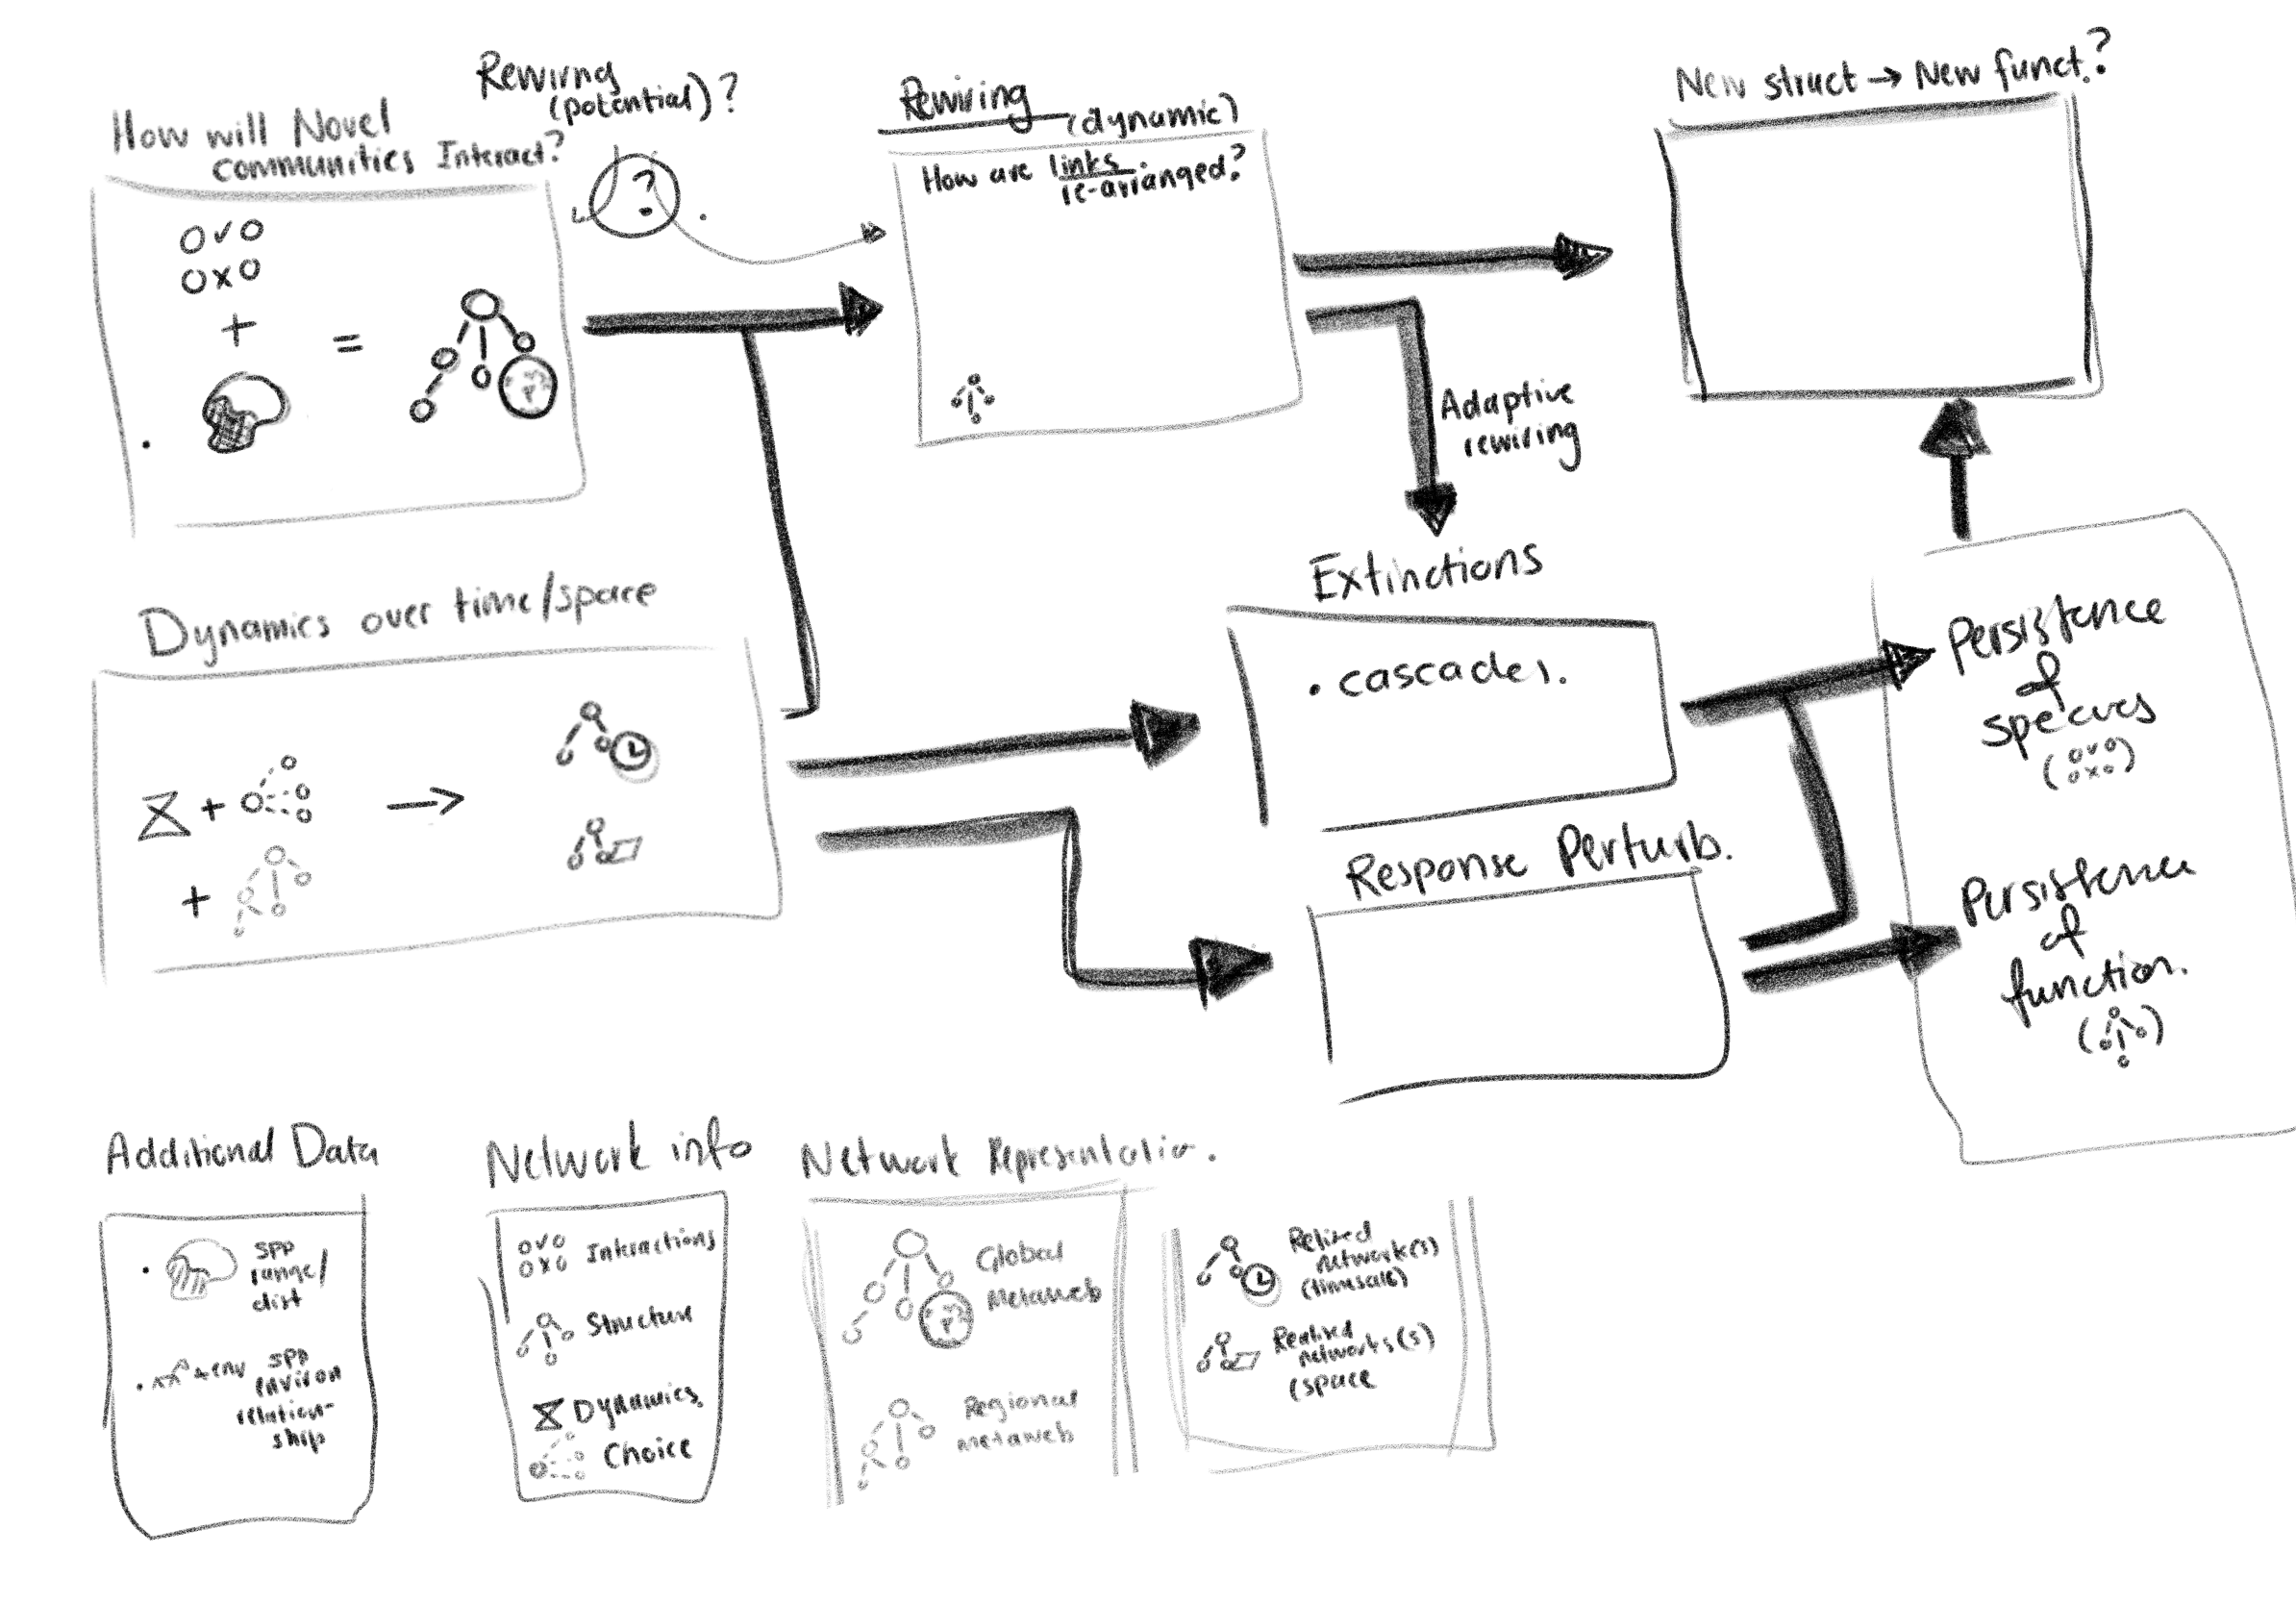
\includegraphics[keepaspectratio]{images/NetworkFuture.png}}

}

\caption{\label{fig-future}Here we highlight some of the outstanding
questions in both network as well as general ecology, as well as some of
the outstanding methodological challenges with regards to constructing
food webs (shown in orange) that we are faced with.}

\end{figure}%

\begin{longtable}[]{@{}
  >{\raggedright\arraybackslash}p{(\linewidth - 4\tabcolsep) * \real{0.2500}}
  >{\raggedright\arraybackslash}p{(\linewidth - 4\tabcolsep) * \real{0.3611}}
  >{\raggedright\arraybackslash}p{(\linewidth - 4\tabcolsep) * \real{0.3889}}@{}}
\caption{This table represents an alternative approach to try and think
about mapping questions to the different network
representations.}\tabularnewline
\toprule\noalign{}
\begin{minipage}[b]{\linewidth}\raggedright
Question (broad)
\end{minipage} & \begin{minipage}[b]{\linewidth}\raggedright
Question (specific)
\end{minipage} & \begin{minipage}[b]{\linewidth}\raggedright
Network representation
\end{minipage} \\
\midrule\noalign{}
\endfirsthead
\toprule\noalign{}
\begin{minipage}[b]{\linewidth}\raggedright
Question (broad)
\end{minipage} & \begin{minipage}[b]{\linewidth}\raggedright
Question (specific)
\end{minipage} & \begin{minipage}[b]{\linewidth}\raggedright
Network representation
\end{minipage} \\
\midrule\noalign{}
\endhead
\bottomrule\noalign{}
\endlastfoot
Species invasions & What species will the invading species interact
with? & Regional metaweb but need to derive information from a global
metaweb since these are interactions that are `novel' \\
Species invasions & How does the invading species alter network dynamics
and function? & Realised network (after having moved through the global
metaweb to understand which interactions are feasible) \\
Range shifts and novel communities & Under global change how will novel
community assemblages interact? & Global metaweb, need context of
broader community \\
Extinctions & Cascading effect of the loss of a species from the network
& Regional metaweb - need to account for entire diet, a realised network
will exclude the entire diet but will allow to elucidate the final
structure \\
Species/community persistence & Dynamics over time.
Stability/resilience. How does a change in pop \emph{A} affect pop
\emph{B}? & Realised networks - but dynamic! \\
Synthetic networks & Creating ecologically plausible communities for
synthetic analyses & Structural networks - data light! \\
Practical use & What is both attainable (data constraints) but also of
practical use to `real world' decision making. So moving from theory to
applied & ??Regional metawebs?? \\
\end{longtable}

\section{Concluding remarks}\label{concluding-remarks}

Having a clear understanding of the interplay between network
representations and the processes that they are capable of encoding is
critical if we are to understand exactly which networks can be used to
answer which questions. As we highlight in Box 1 the different network
representations have different potential uses and it should be clear
that there is no `best' network representation but rather a network
representation that is best suited to its intended purpose. In providing
a formalisation regards to the assumptions, scales, and mechanisms that
need to be explicitly taken into consideration when deciding to use (and
construct) networks we hope to prevent the unintentional misuse or
misinterpretation of networks as well as provide a starting point from
which we can develop a better framework for the applied use of networks
to answer questions that are not only pressing within the field but also
within broader biodiversity science.

\section*{References}\label{references}
\addcontentsline{toc}{section}{References}

\phantomsection\label{refs}
\begin{CSLReferences}{1}{0}
\bibitem[\citeproctext]{ref-allesinaGeneralModelFood2008}
Allesina, S., Alonso, D., \& Pascual, M. (2008). A {General Model} for
{Food Web Structure}. \emph{Science}, \emph{320}(5876), 658--661.
\url{https://doi.org/10.1126/science.1156269}

\bibitem[\citeproctext]{ref-allesinaFoodWebModels2009}
Allesina, S., \& Pascual, M. (2009). Food web models: A plea for groups.
\emph{Ecology Letters}, \emph{12}(7), 652--662.
\url{https://doi.org/10.1111/j.1461-0248.2009.01321.x}

\bibitem[\citeproctext]{ref-banvilleDecipheringProbabilisticSpecies2024}
Banville, F., Strydom, T., Blyth, P., Brimacombe, C., Catchen, M. D.,
Dansereau, G., Higino, G., Malpas, T., Mayall, H., Norman, K., Gravel,
D., \& Poisot, T. (2024). \emph{Deciphering probabilistic species
interaction networks}. EcoEvoRxiv. \url{https://doi.org/10.32942/X28G8Z}

\bibitem[\citeproctext]{ref-beckerOptimisingPredictiveModels2022}
Becker, D. J., Albery, G. F., Sjodin, A. R., Poisot, T., Bergner, L. M.,
Chen, B., Cohen, L. E., Dallas, T. A., Eskew, E. A., Fagre, A. C.,
Farrell, M. J., Guth, S., Han, B. A., Simmons, N. B., Stock, M.,
Teeling, E. C., \& Carlson, C. J. (2022). Optimising predictive models
to prioritise viral discovery in zoonotic reservoirs. \emph{The Lancet
Microbe}, \emph{3}(8), e625--e637.
\url{https://doi.org/10.1016/S2666-5247(21)00245-7}

\bibitem[\citeproctext]{ref-beckermanForagingBiologyPredicts2006}
Beckerman, A. P., Petchey, O. L., \& Warren, P. H. (2006). Foraging
biology predicts food web complexity. \emph{Proceedings of the National
Academy of Sciences}, \emph{103}(37), 13745--13749.
\url{https://doi.org/10.1073/pnas.0603039103}

\bibitem[\citeproctext]{ref-benadiQuantitativePredictionInteractions2022}
Benadi, G., Dormann, C. F., Fründ, J., Stephan, R., \& Vázquez, D. P.
(2022). Quantitative {Prediction} of {Interactions} in {Bipartite
Networks Based} on {Traits}, {Abundances}, and {Phylogeny}. \emph{The
American Naturalist}, \emph{199}(6), 841--854.
\url{https://doi.org/10.1086/714420}

\bibitem[\citeproctext]{ref-berlowGoldilocksFactorFood2008}
Berlow, E. L., Brose, U., \& Martinez, N. D. (2008). The {``{Goldilocks}
factor''} in food webs. \emph{Proceedings of the National Academy of
Sciences}, \emph{105}(11), 4079--4080.
\url{https://doi.org/10.1073/pnas.0800967105}

\bibitem[\citeproctext]{ref-berlowInteractionStrengthsFood2004}
Berlow, E. L., Neutel, A.-M., Cohen, J. E., de Ruiter, P. C., Ebenman,
B., Emmerson, M., Fox, J. W., Jansen, V. A. A., Iwan Jones, J.,
Kokkoris, G. D., Logofet, D. O., McKane, A. J., Montoya, J. M., \&
Petchey, O. (2004). Interaction strengths in food webs: Issues and
opportunities. \emph{Journal of Animal Ecology}, \emph{73}(3), 585--598.
\url{https://doi.org/10.1111/j.0021-8790.2004.00833.x}

\bibitem[\citeproctext]{ref-bitonInductiveLinkPrediction2024}
Biton, B., Puzis, R., \& Pilosof, S. (2024). \emph{Inductive link
prediction boosts data availability and enables cross-community link
prediction in ecological networks}.

\bibitem[\citeproctext]{ref-blanchetCooccurrenceNotEvidence2020}
Blanchet, F. G., Cazelles, K., \& Gravel, D. (2020). Co-occurrence is
not evidence of ecological interactions. \emph{Ecology Letters},
\emph{23}(7), 1050--1063. \url{https://doi.org/10.1111/ele.13525}

\bibitem[\citeproctext]{ref-bluthgenWhyNetworkAnalysis2010}
Blüthgen, N. (2010). Why network analysis is often disconnected from
community ecology: {A} critique and an ecologist's guide. \emph{Basic
and Applied Ecology}, \emph{11}(3), 185--195.
\url{https://doi.org/10.1016/j.baae.2010.01.001}

\bibitem[\citeproctext]{ref-bluthgenEcologyMammalsInteraction2021}
Blüthgen, N., \& Staab, M. (2021). Ecology: {Mammals}, interaction
networks and the relevance of scale. \emph{Current Biology},
\emph{31}(13), R850--R853.
\url{https://doi.org/10.1016/j.cub.2021.05.032}

\bibitem[\citeproctext]{ref-bluthgenCriticalEvaluationNetwork2024}
Blüthgen, N., \& Staab, M. (2024). A {Critical Evaluation} of {Network
Approaches} for {Studying Species Interactions}. \emph{Annual Review of
Ecology, Evolution, and Systematics}, \emph{55}(1), 65--88.
\url{https://doi.org/10.1146/annurev-ecolsys-102722-021904}

\bibitem[\citeproctext]{ref-brimacombeInferredSeasonalInteraction2021}
Brimacombe, C., Bodner, K., \& Fortin, M.-J. (2021). Inferred seasonal
interaction rewiring of a freshwater stream fish network.
\emph{Ecography}, \emph{44}(2), 219--230.
\url{https://doi.org/10.1111/ecog.05452}

\bibitem[\citeproctext]{ref-brimacombeApplyingMethodIts2024}
Brimacombe, C., Bodner, K., \& Fortin, M.-J. (2024). \emph{Applying a
method before its proof-of-concept: {A} cautionary tale using inferred
food webs}. \url{https://doi.org/10.13140/RG.2.2.22076.65927}

\bibitem[\citeproctext]{ref-brimacombeShortcomingsReusingSpecies2023}
Brimacombe, C., Bodner, K., Michalska-Smith, M., Poisot, T., \& Fortin,
M.-J. (2023). Shortcomings of reusing species interaction networks
created by different sets of researchers. \emph{PLOS Biology},
\emph{21}(4), e3002068.
\url{https://doi.org/10.1371/journal.pbio.3002068}

\bibitem[\citeproctext]{ref-brownMetabolicTheoryEcology2004}
Brown, J. H., Gillooly, J. F., Allen, A. P., Savage, V. M., \& West, G.
B. (2004). Toward a {Metabolic Theory} of {Ecology}. \emph{Ecology},
\emph{85}(7), 1771--1789. \url{https://doi.org/10.1890/03-9000}

\bibitem[\citeproctext]{ref-bucheMultitrophicHigherOrderInteractions2024}
Buche, L., Bartomeus, I., \& Godoy, O. (2024). Multitrophic
{Higher-Order Interactions Modulate Species Persistence}. \emph{The
American Naturalist}, \emph{203}(4), 458--472.
\url{https://doi.org/10.1086/729222}

\bibitem[\citeproctext]{ref-canardEmergenceStructuralPatterns2012}
Canard, E., Mouquet, N., Marescot, L., Gaston, K. J., Gravel, D., \&
Mouillot, D. (2012). Emergence of {Structural Patterns} in {Neutral
Trophic Networks}. \emph{PLOS ONE}, \emph{7}(8), e38295.
\url{https://doi.org/10.1371/journal.pone.0038295}

\bibitem[\citeproctext]{ref-caronTraitmatchingModelsPredict2024}
Caron, D., Brose, U., Lurgi, M., Blanchet, F. G., Gravel, D., \&
Pollock, L. J. (2024). Trait-matching models predict pairwise
interactions across regions, not food web properties. \emph{Global
Ecology and Biogeography}, \emph{33}(4), e13807.
\url{https://doi.org/10.1111/geb.13807}

\bibitem[\citeproctext]{ref-caronAddressingEltonianShortfall2022}
Caron, D., Maiorano, L., Thuiller, W., \& Pollock, L. J. (2022).
Addressing the {Eltonian} shortfall with trait-based interaction models.
\emph{Ecology Letters}, \emph{25}(4), 889--899.
\url{https://doi.org/10.1111/ele.13966}

\bibitem[\citeproctext]{ref-catchenMissingLinkDiscerning2023}
Catchen, M. D., Poisot, T., Pollock, L. J., \& Gonzalez, A. (2023).
\emph{The missing link: Discerning true from false negatives when
sampling species interaction networks}.

\bibitem[\citeproctext]{ref-cherifEnvironmentRescueCan2024}
Cherif, M., Brose, U., Hirt, M. R., Ryser, R., Silve, V., Albert, G.,
Arnott, R., Berti, E., Cirtwill, A., Dyer, A., Gauzens, B., Gupta, A.,
Ho, H.-C., Portalier, S. M. J., Wain, D., \& Wootton, K. (2024). The
environment to the rescue: Can physics help predict predator--prey
interactions? \emph{Biological Reviews}, \emph{138}(n/a).
\url{https://doi.org/10.1111/brv.13105}

\bibitem[\citeproctext]{ref-cirtwillQuantitativeFrameworkInvestigating2019}
Cirtwill, A. R., Eklf, A., Roslin, T., Wootton, K., \& Gravel, D.
(2019). A quantitative framework for investigating the reliability of
empirical network construction. \emph{Methods in Ecology and Evolution},
\emph{10}(6), 902--911. \url{https://doi.org/10.1111/2041-210X.13180}

\bibitem[\citeproctext]{ref-cleggImpactIntraspecificVariation2018}
Clegg, T., Ali, M., \& Beckerman, A. P. (2018). The impact of
intraspecific variation on food web structure. \emph{Ecology},
\emph{99}(12), 2712--2720. \url{https://doi.org/10.1002/ecy.2523}

\bibitem[\citeproctext]{ref-curtsdotterEcosystemFunctionPredator2019}
Curtsdotter, A., Banks, H. T., Banks, J. E., Jonsson, M., Jonsson, T.,
Laubmeier, A. N., Traugott, M., \& Bommarco, R. (2019). Ecosystem
function in predator--prey food webs---confronting dynamic models with
empirical data. \emph{Journal of Animal Ecology}, \emph{88}(2),
196--210. \url{https://doi.org/10.1111/1365-2656.12892}

\bibitem[\citeproctext]{ref-dallarivaExploringEvolutionarySignature2016}
Dalla Riva, G. V., \& Stouffer, D. B. (2016). Exploring the evolutionary
signature of food webs' backbones using functional traits. \emph{Oikos},
\emph{125}(4), 446--456. \url{https://doi.org/10.1111/oik.02305}

\bibitem[\citeproctext]{ref-dallasPredictingCrypticLinks2017}
Dallas, T., Park, A. W., \& Drake, J. M. (2017). Predicting cryptic
links in host-parasite networks. \emph{PLOS Computational Biology},
\emph{13}(5), e1005557.
\url{https://doi.org/10.1371/journal.pcbi.1005557}

\bibitem[\citeproctext]{ref-dansereauSpatiallyExplicitPredictions2024}
Dansereau, G., Barros, C., \& Poisot, T. (2024). Spatially explicit
predictions of food web structure from regional-level data.
\emph{Philosophical Transactions of the Royal Society B: Biological
Sciences}, \emph{379}(1909).
\url{https://doi.org/10.1098/rstb.2023.0166}

\bibitem[\citeproctext]{ref-delmasAnalysingEcologicalNetworks2019}
Delmas, E., Besson, M., Brice, M.-H., Burkle, L. A., Riva, G. V. D.,
Fortin, M.-J., Gravel, D., Guimarães, P. R., Hembry, D. H., Newman, E.
A., Olesen, J. M., Pires, M. M., Yeakel, J. D., \& Poisot, T. (2019).
Analysing ecological networks of species interactions. \emph{Biological
Reviews}, \emph{94}(1), 16--36. \url{https://doi.org/10.1111/brv.12433}

\bibitem[\citeproctext]{ref-delmasSimulationsBiomassDynamics2017}
Delmas, E., Brose, U., Gravel, D., Stouffer, D. B., \& Poisot, T.
(2017). Simulations of biomass dynamics in community food webs.
\emph{Methods in Ecology and Evolution}, \emph{8}(7), 881--886.
\url{https://doi.org/10.1111/2041-210X.12713}

\bibitem[\citeproctext]{ref-desjardins-proulxEcologicalInteractionsNetflix2017}
Desjardins-Proulx, P., Laigle, I., Poisot, T., \& Gravel, D. (2017).
Ecological interactions and the {Netflix} problem. \emph{PeerJ},
\emph{5}, e3644. \url{https://doi.org/10.7717/peerj.3644}

\bibitem[\citeproctext]{ref-dormannRisePossibleFall2023}
Dormann, C. F. (2023). The rise, and possible fall, of network ecology.
In \emph{Defining {Agroecology} -- {A Festschrift} for {Teja
Tscharntke}} (pp. 143--159.). Tredition.

\bibitem[\citeproctext]{ref-dunhillExtinctionCascadesCommunity2024}
Dunhill, A. M., Zarzyczny, K., Shaw, J. O., Atkinson, J. W., Little, C.
T. S., \& Beckerman, A. P. (2024). Extinction cascades, community
collapse, and recovery across a {Mesozoic} hyperthermal event.
\emph{Nature Communications}, \emph{15}(1), 8599.
\url{https://doi.org/10.1038/s41467-024-53000-2}

\bibitem[\citeproctext]{ref-dunneNetworkStructureFood2006}
Dunne, J. A. (2006). The {Network Structure} of {Food Webs}. In J. A.
Dunne \& M. Pascual (Eds.), \emph{Ecological networks: {Linking}
structure and dynamics} (pp. 27--86). Oxford University Press.

\bibitem[\citeproctext]{ref-dunneCompilationNetworkAnalyses2008}
Dunne, J. A., Williams, R. J., Martinez, N. D., Wood, R. A., \& Erwin,
D. H. (2008). Compilation and {Network Analyses} of {Cambrian Food
Webs}. \emph{PLOS Biology}, \emph{6}(4), e102.
\url{https://doi.org/10.1371/journal.pbio.0060102}

\bibitem[\citeproctext]{ref-eklofSecondaryExtinctionsFood2013}
Eklöf, A., Tang, S., \& Allesina, S. (2013). Secondary extinctions in
food webs: A {Bayesian} network approach. \emph{Methods in Ecology and
Evolution}, \emph{4}(8), 760--770.
\url{https://doi.org/10.1111/2041-210X.12062}

\bibitem[\citeproctext]{ref-estayEditorialPatternsProcesses2023}
Estay, S. A., Fortin, M.-J., \& López, D. N. (2023). Editorial:
{Patterns} and processes in ecological networks over space.
\emph{Frontiers in Ecology and Evolution}, \emph{11}.

\bibitem[\citeproctext]{ref-fortinNetworkEcologyDynamic2021}
Fortin, M.-J., Dale, M. R. T., \& Brimacombe, C. (2021). Network ecology
in dynamic landscapes. \emph{Proceedings of the Royal Society B:
Biological Sciences}, \emph{288}(1949), rspb.2020.1889, 20201889.
\url{https://doi.org/10.1098/rspb.2020.1889}

\bibitem[\citeproctext]{ref-frickeCollapseTerrestrialMammal2022}
Fricke, E. C., Hsieh, C., Middleton, O., Gorczynski, D., Cappello, C.
D., Sanisidro, O., Rowan, J., Svenning, J.-C., \& Beaudrot, L. (2022).
Collapse of terrestrial mammal food webs since the {Late Pleistocene}.
\emph{Science}, \emph{377}(6609), 1008--1011.
\url{https://doi.org/10.1126/science.abn4012}

\bibitem[\citeproctext]{ref-galianaSpatialScalingSpecies2018}
Galiana, N., Lurgi, M., Claramunt-López, B., Fortin, M.-J., Leroux, S.,
Cazelles, K., Gravel, D., \& Montoya, J. M. (2018). The spatial scaling
of species interaction networks. \emph{Nature Ecology \& Evolution},
\emph{2}(5), 782--790. \url{https://doi.org/10.1038/s41559-018-0517-3}

\bibitem[\citeproctext]{ref-garcia-callejasNonrandomInteractionsGuilds2023}
García-Callejas, D., Godoy, O., Buche, L., Hurtado, M., Lanuza, J. B.,
Allen-Perkins, A., \& Bartomeus, I. (2023). Non-random interactions
within and across guilds shape the potential to coexist in multi-trophic
ecological communities. \emph{Ecology Letters}, \emph{26}(6), 831--842.
\url{https://doi.org/10.1111/ele.14206}

\bibitem[\citeproctext]{ref-golubskiModifyingModifiersWhat2011}
Golubski, A. J., \& Abrams, P. A. (2011). Modifying modifiers: What
happens when interspecific interactions interact? \emph{Journal of
Animal Ecology}, \emph{80}(5), 1097--1108.
\url{https://doi.org/10.1111/j.1365-2656.2011.01852.x}

\bibitem[\citeproctext]{ref-gomezEcologicalInteractionsAre2010}
Gómez, J. M., Verdú, M., \& Perfectti, F. (2010). Ecological
interactions are evolutionarily conserved across the entire tree of
life. \emph{Nature}, \emph{465}(7300), 918--921.
\url{https://doi.org/10.1038/nature09113}

\bibitem[\citeproctext]{ref-gravelBringingEltonGrinnell2019}
Gravel, D., Baiser, B., Dunne, J. A., Kopelke, J.-P., Martinez, N. D.,
Nyman, T., Poisot, T., Stouffer, D. B., Tylianakis, J. M., Wood, S. A.,
\& Roslin, T. (2019). Bringing {Elton} and {Grinnell} together: A
quantitative framework to represent the biogeography of ecological
interaction networks. \emph{Ecography}, \emph{42}(3), 401--415.
\url{https://doi.org/10.1111/ecog.04006}

\bibitem[\citeproctext]{ref-grayJoiningDotsAutomated2015}
Gray, C., Figueroa, D. H., Hudson, L. N., Ma, A., Perkins, D., \&
Woodward, G. (2015). Joining the dots: {An} automated method for
constructing food webs from compendia of published interactions.
\emph{Food Webs}, \emph{5}, 11--20.
\url{https://doi.org/10.1016/j.fooweb.2015.09.001}

\bibitem[\citeproctext]{ref-higinoMismatchIUCNRange2023}
Higino, G. T., Banville, F., Dansereau, G., Muñoz, N. R. F., Windsor,
F., \& Poisot, T. (2023). Mismatch between {IUCN} range maps and species
interactions data illustrated using the {Serengeti} food web.
\emph{PeerJ}, \emph{11}, e14620.
\url{https://doi.org/10.7717/peerj.14620}

\bibitem[\citeproctext]{ref-huiHowInvadeEcological2019}
Hui, C., \& Richardson, D. M. (2019). How to {Invade} an {Ecological
Network}. \emph{Trends in Ecology \& Evolution}, \emph{34}(2), 121--131.
\url{https://doi.org/10.1016/j.tree.2018.11.003}

\bibitem[\citeproctext]{ref-hutchinsonSeeingForestTrees2019}
Hutchinson, M. C., Bramon Mora, B., Pilosof, S., Barner, A. K., Kéfi,
S., Thébault, E., Jordano, P., \& Stouffer, D. B. (2019). Seeing the
forest for the trees: {Putting} multilayer networks to work for
community ecology. \emph{Functional Ecology}, \emph{33}(2), 206--217.
\url{https://doi.org/10.1111/1365-2435.13237}

\bibitem[\citeproctext]{ref-jordanoChasingEcologicalInteractions2016}
Jordano, P. (2016a). Chasing {Ecological Interactions}. \emph{PLOS
Biology}, \emph{14}(9), e1002559.
\url{https://doi.org/10.1371/journal.pbio.1002559}

\bibitem[\citeproctext]{ref-jordanoSamplingNetworksEcological2016}
Jordano, P. (2016b). Sampling networks of ecological interactions.
\emph{Functional Ecology}. \url{https://doi.org/10.1111/1365-2435.12763}

\bibitem[\citeproctext]{ref-kamaruDisruptionAntplantMutualism2024}
Kamaru, D. N., Palmer, T. M., Riginos, C., Ford, A. T., Belnap, J.,
Chira, R. M., Githaiga, J. M., Gituku, B. C., Hays, B. R., Kavwele, C.
M., Kibungei, A. K., Lamb, C. T., Maiyo, N. J., Milligan, P. D.,
Mutisya, S., Ng'weno, C. C., Ogutu, M., Pietrek, A. G., Wildt, B. T., \&
Goheen, J. R. (2024). Disruption of an ant-plant mutualism shapes
interactions between lions and their primary prey. \emph{Science},
\emph{383}(6681), 433--438.
\url{https://doi.org/10.1126/science.adg1464}

\bibitem[\citeproctext]{ref-kefiNetworkStructureFood2015}
Kéfi, S., Berlow, E. L., Wieters, E. A., Joppa, L. N., Wood, S. A.,
Brose, U., \& Navarrete, S. A. (2015). Network structure beyond food
webs: Mapping non-trophic and trophic interactions on {Chilean} rocky
shores. \emph{Ecology}, \emph{96}(1), 291--303.
\url{https://doi.org/10.1890/13-1424.1}

\bibitem[\citeproctext]{ref-kefiMoreMealIntegrating2012}
Kéfi, S., Berlow, E. L., Wieters, E. A., Navarrete, S. A., Petchey, O.
L., Wood, S. A., Boit, A., Joppa, L. N., Lafferty, K. D., Williams, R.
J., Martinez, N. D., Menge, B. A., Blanchette, C. A., Iles, A. C., \&
Brose, U. (2012). More than a meal{\ldots{}} integrating non-feeding
interactions into food webs: {More} than a meal {\ldots{}}.
\emph{Ecology Letters}, \emph{15}(4), 291--300.
\url{https://doi.org/10.1111/j.1461-0248.2011.01732.x}

\bibitem[\citeproctext]{ref-keyesSynthesisingRelationshipsFood2024}
Keyes, A. A., Barner, A. K., \& Dee, L. E. (2024). Synthesising the
{Relationships Between Food Web Structure} and {Robustness}.
\emph{Ecology Letters}, \emph{27}(10), e14533.
\url{https://doi.org/10.1111/ele.14533}

\bibitem[\citeproctext]{ref-krauseCompartmentsRevealedFoodweb2003}
Krause, A. E., Frank, K. A., Mason, D. M., Ulanowicz, R. E., \& Taylor,
W. W. (2003). Compartments revealed in food-web structure.
\emph{Nature}, \emph{426}(6964), 282--285.
\url{https://doi.org/10.1038/nature02115}

\bibitem[\citeproctext]{ref-laenderCarbonTransferHerbivore2010}
Laender, F. D., Oevelen, D. V., Soetaert, K., \& Middelburg, J. J.
(2010). Carbon transfer in a herbivore- and microbial loop-dominated
pelagic food webs in the southern {Barents Sea} during spring and
summer. \emph{Marine Ecology Progress Series}, \emph{398}, 93--107.
\url{https://doi.org/10.3354/meps08335}

\bibitem[\citeproctext]{ref-lajaaitiEcologicalNetworksDynamicsJlJulia2024}
Lajaaiti, I., Bonnici, I., Kéfi, S., Mayall, H., Danet, A., Beckerman,
A. P., Malpas, T., \& Delmas, E. (2024).
\emph{{EcologicalNetworksDynamics}.jl {A Julia} package to simulate the
temporal dynamics of complex ecological networks} (p.
2024.03.20.585899). bioRxiv.
\url{https://doi.org/10.1101/2024.03.20.585899}

\bibitem[\citeproctext]{ref-lindemanTrophicDynamicAspectEcology1942}
Lindeman, R. L. (1942). The {Trophic-Dynamic Aspect} of {Ecology}.
\emph{Ecology}, \emph{23}(4), 399--417.
\url{https://doi.org/10.2307/1930126}

\bibitem[\citeproctext]{ref-llewelynPredictingPredatorPrey2023}
Llewelyn, J., Strona, G., Dickman, C. R., Greenville, A. C., Wardle, G.
M., Lee, M. S. Y., Doherty, S., Shabani, F., Saltré, F., \& Bradshaw, C.
J. A. (2023). Predicting predator--prey interactions in terrestrial
endotherms using random forest. \emph{Ecography}, \emph{2023}(9),
e06619. \url{https://doi.org/10.1111/ecog.06619}

\bibitem[\citeproctext]{ref-momalTreebasedInferenceSpecies2020}
Momal, R., Robin, S., \& Ambroise, C. (2020). Tree-based inference of
species interaction networks from abundance data. \emph{Methods in
Ecology and Evolution}, \emph{11}(5), 621--632.
\url{https://doi.org/10.1111/2041-210X.13380}

\bibitem[\citeproctext]{ref-moralesEffectSpacePlant2008}
Morales, J. M., \& Vázquez, D. P. (2008). The effect of space in
plant--animal mutualistic networks: Insights from a simulation study.
\emph{Oikos}, \emph{117}(9), 1362--1370.
\url{https://doi.org/10.1111/j.0030-1299.2008.16737.x}

\bibitem[\citeproctext]{ref-morales-castillaInferringBioticInteractions2015}
Morales-Castilla, I., Matias, M. G., Gravel, D., \& Araújo, M. B.
(2015). Inferring biotic interactions from proxies. \emph{Trends in
Ecology \& Evolution}, \emph{30}(6), 347--356.
\url{https://doi.org/10.1016/j.tree.2015.03.014}

\bibitem[\citeproctext]{ref-moulatletScalingTrophicSpecialization2024}
Moulatlet, G., Luna, P., Dattilo, W., \& Villalobos, F. (2024).
\emph{The scaling of trophic specialization in interaction networks
across levels of organization}. Authorea.
\url{https://doi.org/10.22541/au.172977303.33335171/v1}

\bibitem[\citeproctext]{ref-olivierExploringTemporalVariability2019}
Olivier, P., Frelat, R., Bonsdorff, E., Kortsch, S., Kröncke, I.,
Möllmann, C., Neumann, H., Sell, A. F., \& Nordström, M. C. (2019).
Exploring the temporal variability of a food web using long-term
biomonitoring data. \emph{Ecography}, \emph{42}(12), 2107--2121.
\url{https://doi.org/10.1111/ecog.04461}

\bibitem[\citeproctext]{ref-pawarDimensionalityConsumerSearch2012}
Pawar, S., Dell, A. I., \& Savage, V. M. (2012). Dimensionality of
consumer search space drives trophic interaction strengths.
\emph{Nature}, \emph{486}(7404), 485--489.
\url{https://doi.org/10.1038/nature11131}

\bibitem[\citeproctext]{ref-petcheySizeForagingFood2008}
Petchey, O. L., Beckerman, A. P., Riede, J. O., \& Warren, P. H. (2008).
Size, foraging, and food web structure. \emph{Proceedings of the
National Academy of Sciences}, \emph{105}(11), 4191--4196.
\url{https://doi.org/10.1073/pnas.0710672105}

\bibitem[\citeproctext]{ref-petcheyFitEfficiencyBiology2011}
Petchey, O. L., Beckerman, A. P., Riede, J. O., \& Warren, P. H. (2011).
Fit, efficiency, and biology: {Some} thoughts on judging food web
models. \emph{Journal of Theoretical Biology}, \emph{279}(1), 169--171.
\url{https://doi.org/10.1016/j.jtbi.2011.03.019}

\bibitem[\citeproctext]{ref-pichlerMachineLearningAlgorithms2020}
Pichler, M., Boreux, V., Klein, A.-M., Schleuning, M., \& Hartig, F.
(2020). Machine learning algorithms to infer trait-matching and predict
species interactions in ecological networks. \emph{Methods in Ecology
and Evolution}, \emph{11}(2), 281--293.
\url{https://doi.org/10.1111/2041-210X.13329}

\bibitem[\citeproctext]{ref-pilosofMultilayerNatureEcological2017}
Pilosof, S., Porter, M. A., Pascual, M., \& Kéfi, S. (2017). The
multilayer nature of ecological networks. \emph{Nature Ecology \&
Evolution}, \emph{1}(4), 101.
\url{https://doi.org/10.1038/s41559-017-0101}

\bibitem[\citeproctext]{ref-poelenGlobalBioticInteractions2014}
Poelen, J. H., Simons, J. D., \& Mungall, C. J. (2014). Global biotic
interactions: {An} open infrastructure to share and analyze
species-interaction datasets. \emph{Ecological Informatics}, \emph{24},
148--159. \url{https://doi.org/10.1016/j.ecoinf.2014.08.005}

\bibitem[\citeproctext]{ref-poisotGuidelinesPredictionSpecies2023}
Poisot, T. (2023). Guidelines for the prediction of species interactions
through binary classification. \emph{Methods in Ecology and Evolution},
\emph{14}(5), 1333--1345. \url{https://doi.org/10.1111/2041-210X.14071}

\bibitem[\citeproctext]{ref-poisotMangalMakingEcological2016}
Poisot, T., Baiser, B., Dunne, J., Kéfi, S., Massol, F., Mouquet, N.,
Romanuk, T. N., Stouffer, D. B., Wood, S. A., \& Gravel, D. (2016).
Mangal -- making ecological network analysis simple. \emph{Ecography},
\emph{39}(4), 384--390. \url{https://doi.org/10.1111/ecog.00976}

\bibitem[\citeproctext]{ref-poisotStructureProbabilisticNetworks2016}
Poisot, T., Cirtwill, A., Cazelles, K., Gravel, D., Fortin, M.-J., \&
Stouffer, D. (2016). The structure of probabilistic networks.
\emph{Methods in Ecology and Evolution}, \emph{7}(3), 303--312.
\url{https://doi.org/10}

\bibitem[\citeproctext]{ref-poisotSpeciesWhyEcological2015}
Poisot, T., Stouffer, D. B., \& Gravel, D. (2015). Beyond species: Why
ecological interaction networks vary through space and time.
\emph{Oikos}, \emph{124}(3), 243--251.
\url{https://doi.org/10.1111/oik.01719}

\bibitem[\citeproctext]{ref-poisotDescribeUnderstandPredict2016}
Poisot, T., Stouffer, D. B., \& Kéfi, S. (2016). Describe, understand
and predict: Why do we need networks in ecology? \emph{Functional
Ecology}, \emph{30}(12), 1878--1882.
\url{https://www.jstor.org/stable/48582345}

\bibitem[\citeproctext]{ref-polisComplexTrophicInteractions1991}
Polis, G. A. (1991). Complex {Trophic Interactions} in {Deserts}: {An
Empirical Critique} of {Food-Web Theory}. \emph{The American
Naturalist}, \emph{138}(1), 123--155.
\url{https://doi.org/10.1086/285208}

\bibitem[\citeproctext]{ref-pollockUnderstandingCooccurrenceModelling2014}
Pollock, L. J., Tingley, R., Morris, W. K., Golding, N., O'Hara, R. B.,
Parris, K. M., Vesk, P. A., \& McCarthy, M. A. (2014). Understanding
co-occurrence by modelling species simultaneously with a {Joint Species
Distribution Model} ({JSDM}). \emph{Methods in Ecology and Evolution},
\emph{5}(5), 397--406. \url{https://doi.org/10.1111/2041-210X.12180}

\bibitem[\citeproctext]{ref-pringleUntanglingFoodWebs2020}
Pringle, R. M. (2020). Untangling {Food Webs}. In \emph{Unsolved
{Problems} in {Ecology}} (pp. 225--238). Princeton University Press.
\url{https://doi.org/10.1515/9780691195322-020}

\bibitem[\citeproctext]{ref-pringleResolvingFoodWebStructure2020}
Pringle, R. M., \& Hutchinson, M. C. (2020). Resolving {Food-Web
Structure}. \emph{Annual Review of Ecology, Evolution and Systematics},
\emph{51}(Volume 51, 2020), 55--80.
\url{https://doi.org/10.1146/annurev-ecolsys-110218-024908}

\bibitem[\citeproctext]{ref-proulxNetworkThinkingEcology2005}
Proulx, S. R., Promislow, D. E. L., \& Phillips, P. C. (2005). Network
thinking in ecology and evolution. \emph{Trends in Ecology \&
Evolution}, \emph{20}(6), 345--353.
\url{https://doi.org/10.1016/j.tree.2005.04.004}

\bibitem[\citeproctext]{ref-pykeOptimalForagingTheory1984}
Pyke, G. (1984). Optimal {Foraging Theory}: {A Critical Review}.
\emph{Annual Review of Ecology, Evolution and Systematic}, \emph{15},
523--575. \url{https://doi.org/10.1146/annurev.ecolsys.15.1.523}

\bibitem[\citeproctext]{ref-quinteroDownscalingMutualisticNetworks2024}
Quintero, E., Arroyo-Correa, B., Isla, J., Rodríguez-Sánchez, F., \&
Jordano, P. (2024). \emph{Downscaling mutualistic networks from species
to individuals reveals consistent interaction niches and roles within
plant populations} (p. 2024.02.02.578595). bioRxiv.
\url{https://doi.org/10.1101/2024.02.02.578595}

\bibitem[\citeproctext]{ref-rooneyLandscapeTheoryFood2008}
Rooney, N., McCann, K. S., \& Moore, J. C. (2008). A landscape theory
for food web architecture. \emph{Ecology Letters}, \emph{11}(8),
867--881. \url{https://doi.org/10.1111/j.1461-0248.2008.01193.x}

\bibitem[\citeproctext]{ref-roopnarineExtinctionCascadesCatastrophe2006}
Roopnarine, P. D. (2006). Extinction {Cascades} and {Catastrophe} in
{Ancient Food Webs}. \emph{Paleobiology}, \emph{32}(1), 1--19.
\url{https://www.jstor.org/stable/4096814}

\bibitem[\citeproctext]{ref-roopnarineEcologicalModellingPaleocommunity2017}
Roopnarine, P. D. (2017). Ecological {Modelling} of {Paleocommunity Food
Webs}. In \emph{Conservation {Paleobiology}: {Using} the {Past} to
{Manage} for the {Future}} (pp. 201--226). University of Chicago Press.

\bibitem[\citeproctext]{ref-saberskiImpactDataResolution2024}
Saberski, E., Lorimer, T., Carpenter, D., Deyle, E., Merz, E., Park, J.,
Pao, G. M., \& Sugihara, G. (2024). The impact of data resolution on
dynamic causal inference in multiscale ecological networks.
\emph{Communications Biology}, \emph{7}(1), 1--10.
\url{https://doi.org/10.1038/s42003-024-07054-z}

\bibitem[\citeproctext]{ref-saraviaEcologicalNetworkAssembly2022}
Saravia, L. A., Marina, T. I., Kristensen, N. P., De Troch, M., \& Momo,
F. R. (2022). Ecological network assembly: {How} the regional metaweb
influences local food webs. \emph{Journal of Animal Ecology},
\emph{91}(3), 630--642. \url{https://doi.org/10.1111/1365-2656.13652}

\bibitem[\citeproctext]{ref-schwarzTemporalScaledependencePlant2020}
Schwarz, B., Vázquez, D. P., CaraDonna, P. J., Knight, T. M., Benadi,
G., Dormann, C. F., Gauzens, B., Motivans, E., Resasco, J., Blüthgen,
N., Burkle, L. A., Fang, Q., Kaiser-Bunbury, C. N., Alarcón, R., Bain,
J. A., Chacoff, N. P., Huang, S.-Q., LeBuhn, G., MacLeod, M., \ldots{}
Fründ, J. (2020). Temporal scale-dependence of plant--pollinator
networks. \emph{Oikos}, \emph{129}(9), 1289--1302.
\url{https://doi.org/10.1111/oik.07303}

\bibitem[\citeproctext]{ref-segarRoleEvolutionShaping2020}
Segar, S. T., Fayle, T. M., Srivastava, D. S., Lewinsohn, T. M., Lewis,
O. T., Novotny, V., Kitching, R. L., \& Maunsell, S. C. (2020). The
{Role} of {Evolution} in {Shaping Ecological Networks}. \emph{Trends in
Ecology \& Evolution}, \emph{35}(5), 454--466.
\url{https://doi.org/10.1016/j.tree.2020.01.004}

\bibitem[\citeproctext]{ref-shawFrameworkReconstructingAncient2024}
Shaw, J. O., Dunhill, A. M., Beckerman, A. P., Dunne, J. A., \& Hull, P.
M. (2024). \emph{A framework for reconstructing ancient food webs using
functional trait data} (p. 2024.01.30.578036). bioRxiv.
\url{https://doi.org/10.1101/2024.01.30.578036}

\bibitem[\citeproctext]{ref-soberonGrinnellianEltonianNiches2007}
Soberón, J. (2007). Grinnellian and {Eltonian} niches and geographic
distributions of species. \emph{Ecology Letters}, \emph{10}(12),
1115--1123. \url{https://doi.org/10.1111/j.1461-0248.2007.01107.x}

\bibitem[\citeproctext]{ref-songRigorousValidationEcological2024}
Song, C., \& Levine, J. M. (2024). \emph{Rigorous (in)validation of
ecological models} (p. 2024.09.19.613075). bioRxiv.
\url{https://doi.org/10.1101/2024.09.19.613075}

\bibitem[\citeproctext]{ref-staniczenkoStructuralDynamicsRobustness2010}
Staniczenko, P. P. A., Lewis, O. T., Jones, N. S., \& Reed-Tsochas, F.
(2010). Structural dynamics and robustness of food webs. \emph{Ecology
Letters}, \emph{13}(7), 891--899.
\url{https://doi.org/10.1111/j.1461-0248.2010.01485.x}

\bibitem[\citeproctext]{ref-stockPairwiseLearningPredicting2021}
Stock, M. (2021). Pairwise learning for predicting pollination
interactions based on traits and phylogeny. \emph{Ecological Modelling},
14.

\bibitem[\citeproctext]{ref-stoufferAllEcologicalModels2019}
Stouffer, D. B. (2019). All ecological models are wrong, but some are
useful. \emph{Journal of Animal Ecology}, \emph{88}(2), 192--195.
\url{https://doi.org/10.1111/1365-2656.12949}

\bibitem[\citeproctext]{ref-strydomFoodWebReconstruction2022}
Strydom, T., Bouskila, S., Banville, F., Barros, C., Caron, D., Farrell,
M. J., Fortin, M.-J., Hemming, V., Mercier, B., Pollock, L. J., Runghen,
R., Dalla Riva, G. V., \& Poisot, T. (2022). Food web reconstruction
through phylogenetic transfer of low-rank network representation.
\emph{Methods in Ecology and Evolution}, \emph{13}(12), 2838--2849.
\url{https://doi.org/10.1111/2041-210X.13835}

\bibitem[\citeproctext]{ref-strydomGraphEmbeddingTransfer2023}
Strydom, T., Bouskila, S., Banville, F., Barros, C., Caron, D., Farrell,
M. J., Fortin, M.-J., Mercier, B., Pollock, L. J., Runghen, R., Dalla
Riva, G. V., \& Poisot, T. (2023). Graph embedding and transfer learning
can help predict potential species interaction networks despite data
limitations. \emph{Methods in Ecology and Evolution}, \emph{14}(12),
2917--2930. \url{https://doi.org/10.1111/2041-210X.14228}

\bibitem[\citeproctext]{ref-strydomRoadmapPredictingSpecies2021}
Strydom, T., Catchen, M. D., Banville, F., Caron, D., Dansereau, G.,
Desjardins-Proulx, P., Forero-Muñoz, N. R., Higino, G., Mercier, B.,
Gonzalez, A., Gravel, D., Pollock, L., \& Poisot, T. (2021). A roadmap
towards predicting species interaction networks (across space and time).
\emph{Philosophical Transactions of the Royal Society B: Biological
Sciences}, \emph{376}(1837), 20210063.
\url{https://doi.org/10.1098/rstb.2021.0063}

\bibitem[\citeproctext]{ref-terryFindingMissingLinks2020}
Terry, J. C. D., \& Lewis, O. T. (2020). Finding missing links in
interaction networks. \emph{Ecology}, \emph{101}(7), e03047.
\url{https://doi.org/10.1002/ecy.3047}

\bibitem[\citeproctext]{ref-valdovinosBioenergeticFrameworkAboveground2023}
Valdovinos, F. S., Hale, K. R. S., Dritz, S., Glaum, P. R., McCann, K.
S., Simon, S. M., Thébault, E., Wetzel, W. C., Wootton, K. L., \&
Yeakel, J. D. (2023). A bioenergetic framework for aboveground
terrestrial food webs. \emph{Trends in Ecology \& Evolution},
\emph{38}(3), 301--312. \url{https://doi.org/10.1016/j.tree.2022.11.004}

\bibitem[\citeproctext]{ref-vandewalleArthropodFoodWebs2023}
Van De Walle, R., Logghe, G., Haas, N., Massol, F., Vandegehuchte, M.
L., \& Bonte, D. (2023). Arthropod food webs predicted from body size
ratios are improved by incorporating prey defensive properties.
\emph{Journal of Animal Ecology}, \emph{92}(4), 913--924.
\url{https://doi.org/10.1111/1365-2656.13905}

\bibitem[\citeproctext]{ref-vazquezUnitingPatternProcess2009}
Vázquez, D. P., Blüthgen, N., Cagnolo, L., \& Chacoff, N. P. (2009).
Uniting pattern and process in plant--animal mutualistic networks: A
review. \emph{Annals of Botany}, \emph{103}(9), 1445--1457.
\url{https://doi.org/10.1093/aob/mcp057}

\bibitem[\citeproctext]{ref-wellsSpeciesInteractionsEstimating2013}
Wells, K., \& O'Hara, R. B. (2013). Species interactions: Estimating
per-individual interaction strength and covariates before simplifying
data into per-species ecological networks. \emph{Methods in Ecology and
Evolution}, \emph{4}(1), 1--8.
\url{https://doi.org/10.1111/j.2041-210x.2012.00249.x}

\bibitem[\citeproctext]{ref-whiteRelationshipsBodySize2007}
White, E. P., Ernest, S. K. M., Kerkhoff, A. J., \& Enquist, B. J.
(2007). Relationships between body size and abundance in ecology.
\emph{Trends in Ecology \& Evolution}, \emph{22}(6), 323--330.
\url{https://doi.org/10.1016/j.tree.2007.03.007}

\bibitem[\citeproctext]{ref-williamsSimpleRulesYield2000}
Williams, R. J., \& Martinez, N. D. (2000). Simple rules yield complex
food webs. \emph{Nature}, \emph{404}(6774), 180--183.
\url{https://doi.org/10.1038/35004572}

\bibitem[\citeproctext]{ref-williamsSuccessItsLimits2008}
Williams, R. J., \& Martinez, N. D. (2008). Success and its limits among
structural models of complex food webs. \emph{Journal of Animal
Ecology}, \emph{77}(3), 512--519.
\url{https://doi.org/10.1111/j.1365-2656.2008.01362.x}

\bibitem[\citeproctext]{ref-windsorUsingEcologicalNetworks2023}
Windsor, F. M., van den Hoogen, J., Crowther, T. W., \& Evans, D. M.
(2023). Using ecological networks to answer questions in global
biogeography and ecology. \emph{Journal of Biogeography}, \emph{50}(1),
57--69. \url{https://doi.org/10.1111/jbi.14447}

\bibitem[\citeproctext]{ref-woottonModularTheoryTrophic2023}
Wootton, K. L., Curtsdotter, A., Roslin, T., Bommarco, R., \& Jonsson,
T. (2023). Towards a modular theory of trophic interactions.
\emph{Functional Ecology}, \emph{37}(1), 26--43.
\url{https://doi.org/10.1111/1365-2435.13954}

\bibitem[\citeproctext]{ref-xieCompletenessCommunityStructure2017}
Xie, J.-R., Zhang, P., Zhang, H.-F., \& Wang, B.-H. (2017). Completeness
of {Community Structure} in {Networks}. \emph{Scientific Reports},
\emph{7}(1), 5269. \url{https://doi.org/10.1038/s41598-017-05585-6}

\bibitem[\citeproctext]{ref-yeakelCollapseEcologicalNetwork2014}
Yeakel, J. D., Pires, M. M., Rudolf, L., Dominy, N. J., Koch, P. L.,
Guimarães, P. R., \& Gross, T. (2014). Collapse of an ecological network
in {Ancient Egypt}. \emph{PNAS}, \emph{111}(40), 14472--14477.
\url{https://doi.org/10.1073/pnas.1408471111}

\bibitem[\citeproctext]{ref-yodzisCompartmentationRealAssembled1982}
Yodzis, P. (1982). The {Compartmentation} of {Real} and {Assembled
Ecosystems}. \emph{The American Naturalist}, \emph{120}(5), 551--570.
\url{https://doi.org/10.1086/284013}

\bibitem[\citeproctext]{ref-yodzisBodySizeConsumerResource1992}
Yodzis, P., \& Innes, S. (1992). Body {Size} and {Consumer-Resource
Dynamics}. \emph{The American Naturalist}, \emph{139}(6), 1151--1175.
\url{https://doi.org/10.1086/285380}

\end{CSLReferences}





\end{document}
